% Pairwise Independence of Internal Splitting, Dichotomy, and Composition
% in Finite Extensional Magmas
% arXiv preprint
\documentclass[sigconf,screen]{acmart}

% Suppress ACM-specific metadata (default placeholders)
\settopmatter{printacmref=false}
\renewcommand\footnotetextcopyrightpermission[1]{}
\pagestyle{plain}
\acmDOI{}
\acmISBN{}
\acmConference[]{}{}{}
\acmYear{2026}
\acmPrice{}

% Lean code listings
\usepackage{listings}
\lstset{
  basicstyle=\ttfamily\small,
  columns=flexible,
  breaklines=true,
  frame=none,
  xleftmargin=1em,
}

% TikZ for independence diagram
\usepackage{tikz}
\usetikzlibrary{arrows.meta,positioning,decorations.markings}

% Shortcuts
\newcommand{\dotop}{\cdot}
\newcommand{\FRM}{\textsf{FRM}}
\newcommand{\ICP}{\textsf{ICP}}
\newcommand{\Fin}{\mathrm{Fin}}
\newcommand{\core}{\mathrm{core}}
\newcommand{\Nat}{\mathbb{N}}

% Additional theorem environments (ACM provides theorem, lemma, corollary, proposition, definition)
\newtheorem{observation}{Observation}
\theoremstyle{remark}
\newtheorem{remark}{Remark}

\begin{document}

\title{Pairwise Independence of Internal Splitting, Dichotomy, and Composition in Finite Extensional Magmas}
\thanks{Preprint version. The Lean proofs, SAT search scripts, and manuscript text were developed with assistance from Claude (Anthropic). All results have been independently verified: Lean proofs compile with \texttt{lake build} (zero \texttt{sorry}), and SAT counterexamples are frozen in the repository for reproducibility. The author takes full responsibility for all contents.}

\author{Stefano Palmieri}
\affiliation{
  \institution{Independent Researcher}
  \city{Austin}
  \state{Texas}
  \country{USA}
}

\keywords{finite extensional magma, pairwise independence, classifier dichotomy, internal composition, Lean~4, machine-checked proofs}

\begin{abstract}
Four obstructions jointly narrow the class of finite magmas that can simultaneously represent, classify, and compose with their own operation: nontrivial combinatory algebras with S and K must be infinite; associativity is incompatible with combining a classifier and a retraction pair; commutativity is incompatible with two distinct left-absorbers; and a single left-absorber collapses any classifier. The setting that survives these narrowings is finite, non-associative, non-commutative, extensional 2-pointed magmas.

We treat the operation $\dotop$ as a fixed structuring relation that is not itself internalizable (a Tarski-style structural limit) and ask what can be internalized within $(A, \dotop)$ as behaviors of its elements. Three internalizations are the paper's main objects: internal splitting~(S) for encoding, internal dichotomy~(D) for binary judgment, and internal composition~(C) for operation chaining. We prove they are pairwise independent. Lean-verified finite counterexamples at sizes $4$ through $10$ establish all six non-implications, four with provably tight bounds. A joint irredundance result strengthens this: all eight Boolean combinations of $(S, D, C)$ are realized, so no capability is reducible to a Boolean function of the other two. The minimum coexistence witness has $N\!=\!5$, which is optimal: ICP requires 3 pairwise distinct core elements, so $N \geq 5$. The three-category decomposition induced by D is an isomorphism invariant; principal coexistence witnesses are role-rigid (trivial automorphism group); and the ICP is logically equivalent to the standard Compose+Inert axioms. Lean-verified results --- independence counterexamples, joint-irredundance witnesses, decomposition invariance, the ICP equivalence, the all-$N$ scaling witness, H-triple type-coherence, and the $N\!=\!5$ structure theorem --- compile with zero \texttt{sorry}; the remaining universal-$N$ algebraic results in Section~\ref{sec:universal} not yet transcribed to Lean have hand proofs supported by Z3 UNSAT certificates.
\end{abstract}

\maketitle

% ══════════════════════════════════════════════════════════════
\section{Introduction}
\label{sec:introduction}
% ══════════════════════════════════════════════════════════════

A finite magma is the Cayley table of a binary operation, stripped of syntax and types. We study three operational capabilities of such a magma --- the operation \emph{representing}, \emph{classifying}, and \emph{composing with} its own structure --- and ask whether they are algebraically independent or whether one forces another. These capabilities have been studied abstractly in the reflection literature~\cite{smith84,brown16}; our contribution is to pin them down as independent algebraic properties in the finite setting. The formal framework is finite extensional 2-pointed magmas: a finite set with a binary operation, exactly two left-absorbers, and row-extensionality~\cite{burris81}.

Four obstructions jointly narrow the candidate class of finite magmas in which all three capabilities can coexist. \emph{(i)} Nontrivial combinatory algebras with $\mathbf{s}$ and $\mathbf{k}$ are necessarily infinite (Theorem~\ref{thm:k-infinity}), ruling out the most direct finite analogues of PCA/TCA-style~\cite{vanoosten08,longley15,bethke88} and Turing-object-style~\cite{cockett08} universality. \emph{(ii)} Associativity is incompatible with combining a classifier and a retraction pair (Theorem~\ref{thm:no-assoc}), excluding semigroups, monoids, groups, and rings. \emph{(iii)} Commutativity is incompatible with two distinct left-absorbers (Theorem~\ref{thm:asymmetry}), forcing the operation to be directed. \emph{(iv)} A single left-absorber collapses any classifier into itself (Proposition~\ref{prop:single-absorber}), forcing at least two absorbers. The setting of this paper --- finite, non-associative, non-commutative, extensional 2-pointed magmas --- is what survives the four narrowings. Within it, we identify three algebraic properties: internal splitting~(S), a section-retraction pair on the non-absorber \emph{core}; the classifier dichotomy~(D), a clean partition of core elements into those whose action on core lands entirely in the absorbers and those whose action avoids them entirely; and the Internal Composition Property~(C), a non-trivial factorization in the left-regular representation restricted to core.

Our main result is that S, D, and C are pairwise independent: no one implies any other. Lean-verified finite counterexamples at sizes $N\!=\!4, 5, 6, 8,$ and $10$ establish all six non-implications; coexistence witnesses at $N\!=\!5$ and $N\!=\!6$ show all three can hold simultaneously. The $N\!=\!5$ bound is optimal: ICP requires 3 pairwise distinct core elements, forcing $|S| \geq 5$. Each counterexample is a concrete Cayley table found by SAT search and independently verified in Lean~4~\cite{moura21}, zero \texttt{sorry}. Whether the independence extends to $\lambda$-calculus or typed settings is an open question (Section~\ref{sec:discussion}).

Beyond independence, we prove several additional structural results. The no-associativity theorem (Theorem~\ref{thm:no-assoc}) rules out the classical algebraic hierarchy: no extensional 2-pointed magma carrying both a classifier and a retraction pair has a right identity or is associative. The three-category decomposition induced by~D is an algebraic invariant (Theorem~\ref{thm:functoriality}); the principal coexistence witnesses are \emph{role-rigid} (Proposition~\ref{prop:witness-rigid}), and at the minimum coexistence size $N\!=\!5$ the roles of retraction, classifier, and C-triple are determined: every retraction pair satisfies $s = r$ (so strong S is unsatisfiable) and every C-triple takes the form $(\tau_1, g, \tau_2)$ for the two classifiers and unique non-classifier (Theorem~\ref{thm:N5-structure}); at $N \geq 6$ strong S re-opens and rigidity fails (Proposition~\ref{prop:N6-nonrigid}). The ICP is equivalent to the standard Compose+Inert axioms (Theorem~\ref{thm:icp-equiv}).

\paragraph{Contributions.}
\begin{enumerate}
  \item Four universal algebraic obstructions that jointly narrow the candidate class to the setting: K-infinity (combinatory algebras must be infinite), no-associativity (the classical algebraic hierarchy is excluded), asymmetry (commutativity incompatible with two absorbers), and single-absorber collapse (one absorber collapses any classifier). A schematic classifier-constancy argument further rules out mediality, left/right self-distributivity, and right identity under D or S+D (Section~\ref{sec:universal}, Proposition~\ref{prop:single-absorber}).
  \item An independence theorem: S, D, and C are pairwise independent, with Lean-verified counterexamples in all six directions at $N\!=\!4$ through $N\!=\!10$ (Section~\ref{sec:independence}), and coexistence witnesses at $N\!=\!5$ and $N\!=\!6$ (Section~\ref{sec:bound}).
  \item An optimal bound: $N\!=\!5$ is the minimum carrier size for S+D+C coexistence. ICP is impossible at $N\!=\!4$ by pigeonhole (Theorem~\ref{thm:no-icp-4}).
  \item Decomposition invariance and role rigidity: the three-category partition is preserved by isomorphisms (Section~\ref{sec:invariance}); the principal coexistence witnesses have trivial automorphism group (Proposition~\ref{prop:witness-rigid}); at $N\!=\!5$ a structure theorem (Theorem~\ref{thm:N5-structure}) forces retraction, classifier, and C-triple onto the three core slots and rules out strong S altogether, while at $N \geq 6$ strong S returns and rigidity fails (Proposition~\ref{prop:N6-nonrigid}): a size-driven phase transition.
  \item A characterization of C confirming the ICP is not ad hoc: it is logically equivalent to Compose+Inert under variable renaming, with necessity of the non-degeneracy conditions demonstrated by Lean-verified witnesses (Section~\ref{sec:icp}).
  \item Joint irredundance: all eight cells of the $(S, D, C)$ Boolean cube are inhabited by Lean-verified witnesses (Section~\ref{sec:boolean-cube}), so no capability is a Boolean function of the other two.
\end{enumerate}

% ══════════════════════════════════════════════════════════════
\section{Definitions}
\label{sec:definitions}
% ══════════════════════════════════════════════════════════════

Throughout, $(S, \dotop)$ is a finite magma on $\Fin(n) = \{0, 1, \ldots, n-1\}$ with binary operation $\dotop : \Fin(n) \times \Fin(n) \to \Fin(n)$.

\begin{definition}[Extensional 2-Pointed Magma]
\label{def:epm}
An \emph{extensional 2-pointed magma} is a tuple $(S, \dotop, z_1, z_2)$ where:
\begin{enumerate}
  \item $z_1, z_2 \in S$ are distinct \emph{left-absorbers}: $z_i \dotop x = z_i$ for all $x$.
  \item No other element is a left-absorber.
  \item \emph{Extensionality}: if $a \dotop x = b \dotop x$ for all $x$, then $a = b$.
\end{enumerate}
We write $\core(S) := S \setminus \{z_1, z_2\}$ for the non-absorber elements.
\end{definition}

Extensionality is the framework's central commitment: an element's identity is exhausted by its row in the Cayley table, so two elements that act identically under the operation are the same element. Type-theoretically, this is \emph{propositional row-extensionality} on the carrier --- an implication from pointwise row equality (a finite, decidable predicate at finite carriers) to carrier equality, taken as an axiom of the definition. The implication is constructively meaningful: at any finite carrier, the antecedent is verifiable by exhaustive comparison, and the consequent is the standard equality on $\Fin(n)$. Every subsequent result in this paper depends on this.

The two-absorber requirement is not a parameter choice but a minimality claim. Two is the minimum for the operation to internally register a binary outcome: with a single absorber, there is nowhere for a complementary outcome to land, and the classifier dichotomy (Definition~\ref{def:cd}) cannot be formulated. Proposition~\ref{prop:single-absorber} below makes this precise: extensionality collapses any would-be classifier into the absorber itself. The axioms fix the count at exactly two so that internal classification is forced without adding extraneous constant rows. The axioms do \emph{not}, however, commit to a stronger reading of the two absorbers as ``opposites'' in any structural sense: the theorems are compatible both with a symmetric reading (two indistinguishable ways the operation fails to discriminate) and a polar reading (two poles of a polarity). This is a genuine freedom in the theory.

\begin{proposition}[Single-Absorber Collapse]
\label{prop:single-absorber}
In any extensional magma $(S, \dotop)$ with a left-absorber $z \in S$, if $\tau \in S$ satisfies $\tau \dotop x = z$ for all $x \in S$, then $\tau = z$. Consequently, reading Definition~\ref{def:cd} with $\{z_1, z_2\}$ replaced by a singleton $\{z\}$ makes the classifier condition unsatisfiable: the requirement $\tau \neq z$ together with $\tau \dotop x \in \{z\}$ for all $x$ has no solution. Two distinct absorbers is the smallest count at which a non-degenerate classifier dichotomy can be formulated.
\end{proposition}

\begin{proof}
The rows $x \mapsto \tau \dotop x$ and $x \mapsto z \dotop x$ are both constantly $z$, so extensionality gives $\tau = z$. The corollary is immediate. Lean: \texttt{single\_absorber\_collapse}.
\end{proof}

\begin{definition}[Faithful Retract Magma]
\label{def:frm}
A \emph{Faithful Retract Magma} $(\FRM)$ extends an extensional 2-pointed magma with a \emph{retraction pair} $s, r \in \core(S)$ satisfying $r \dotop (s \dotop x) = x$ for all $x \in \core(S)$, with $r \dotop z_1 = z_1$ (anchoring). The remaining absorber outputs of $s$ and $r$ are unconstrained.
\end{definition}

\paragraph{Retraction pair convention.}
\label{rem:mutual}
Throughout this paper, the retraction pair $(s, r)$ satisfies the mutual-inverse condition on core: $r \dotop (s \dotop x) = x$ and $s \dotop (r \dotop x) = x$ for all $x \in \core(S)$. This matches the Lean formalization. The choice is load-bearing, not stylistic. One-sided retraction ($r \dotop (s \dotop x) = x$) is a decodable-encoding condition: $s$ produces codes that $r$ can recover. Mutual inverse is the stronger, faithful-representation condition: $s$ and $r$ invert each other in both directions on core, so the encoding neither invents nor loses information. Most theorems (9 of 11) go through under the one-sided hypothesis, and we note this where relevant; two results, retraction pair placement (Theorem~\ref{thm:placement}) and the tight bound $|S| \geq 5$ when $s \neq r$ (Theorem~\ref{thm:card}), genuinely require the full mutual inverse. Proposition~\ref{prop:one-sided-sep} below shows this distinction is non-vacuous: at $N = 4$ there is a concrete one-sided retraction pair with $s \neq r$ that fails mutual inverse, simultaneously confirming that the mutual-inverse hypothesis in Theorem~\ref{thm:card} cannot be weakened.

\begin{proposition}[One-Sided / Mutual-Inverse Separation]
\label{prop:one-sided-sep}
There is an extensional 2-pointed magma on $\Fin(4)$ admitting a one-sided retraction pair $(s, r)$ with $s \neq r$, $s, r \in \core$, $r \dotop z_1 = z_1$, and $r \dotop (s \dotop x) = x$ for all $x \in \core$, but no mutual-inverse pair $(s', r')$ with $s' \neq r'$. The explicit Cayley table (rows indexed by the left operand) is:
\[
\begin{array}{c|cccc}
\dotop & 0 & 1 & 2 & 3 \\ \hline
0 & 0 & 0 & 0 & 0 \\
1 & 1 & 1 & 1 & 1 \\
2 & 1 & 0 & 1 & 3 \\
3 & 0 & 2 & 1 & 3
\end{array}
\]
with $z_1 = 0$, $z_2 = 1$, $s = 2$, $r = 3$. Mutual inverse fails at $x = 2$: $s \dotop (r \dotop 2) = 2 \dotop 1 = 0 \neq 2$. Lean: \texttt{mutual\_strictly\_stronger\_than\_one\_sided}.
\end{proposition}

\begin{proof}
All axioms (two left-absorbers, extensionality, no other zeros, anchoring, one-sided retraction) are verified by direct inspection of the table; the Lean file discharges each check by \texttt{decide}. The non-existence of a mutual-inverse pair with $s' \neq r'$ is also checked by \texttt{decide} over $\Fin(4) \times \Fin(4)$. The separation establishes two points: (i) mutual inverse strictly implies one-sided retraction, so the axiom choice is substantive; (ii) the one-sided analogue of Theorem~\ref{thm:card} with $s \neq r$ would admit this $N = 4$ witness, so the bound $|S| \geq 5$ under mutual inverse cannot be weakened to one-sided.
\end{proof}

The retraction pair provides a section/retraction structure on core: $s$ acts as a section and $r$ as a retraction. In finite witnesses this can be used to organize elements into coding schemes, but we do not assume a canonical global encoding.

\begin{definition}[Classifier Dichotomy]
\label{def:cd}
An extensional 2-pointed magma satisfies the \emph{classifier dichotomy} when:
\begin{enumerate}
  \item A \emph{classifier} $\tau \in \core(S)$ exists with $\tau \dotop x \in \{z_1, z_2\}$ for all $x$.
  \item For every $y \in \core(S)$, either
    \begin{itemize}
      \item $y \dotop x \in \{z_1, z_2\}$ for all $x \in \core(S)$ \quad ($y$ is a \emph{classifier}), or
      \item $y \dotop x \notin \{z_1, z_2\}$ for all $x \in \core(S)$ \quad ($y$ is a \emph{non-classifier}).
    \end{itemize}
  \item At least one non-classifier exists (excluding the degenerate case where the ``dichotomy'' has only one inhabited class).
\end{enumerate}
\end{definition}

The dichotomy creates a three-category decomposition $S = Z \sqcup C \sqcup N$ where $Z = \{z_1, z_2\}$ (absorbers), $C$ (classifiers), and $N$ (non-classifiers). No element can be partially classifying. We call outputs in $\{z_1, z_2\}$ \emph{absorber-valued}.

\begin{definition}[Internal Composition Property]
\label{def:icp}
A magma $(S, \dotop, z_1, z_2)$ satisfies the \emph{Internal Composition Property} $(\ICP)$ when:
\[
\exists\, a, b, c \in \core(S),\ \text{pairwise distinct, such that:}
\]
\begin{enumerate}
  \item \emph{Core-preservation}: $b \dotop x \notin \{z_1, z_2\}$ for all $x \in \core(S)$.
  \item \emph{Factorization}: $a \dotop x = c \dotop (b \dotop x)$ for all $x \in \core(S)$.
  \item \emph{Non-triviality}: $|\{a \dotop x : x \in \core(S)\}| \geq 2$.
\end{enumerate}
\end{definition}

ICP says: the left-regular representation admits a non-trivial factorization on core. One core action factors through two others, one of them core-preserving: a single fragment of internal composition. Equivalently, the ICP is the point at which the operation contains a pattern of its own use as a resource, with some element's row visibly the result of composing the operation with itself through another element. In Section~\ref{sec:icp} we prove that $\ICP$ is equivalent to the standard operational axioms Compose+Inert (Theorem~\ref{thm:icp-equiv}).

\begin{definition}[Capability S]
An extensional 2-pointed magma has capability $S$ (internal splitting) if it admits a retraction pair.
\end{definition}

\begin{definition}[Capability D]
An extensional 2-pointed magma has capability $D$ (internal dichotomy) if it satisfies the classifier dichotomy (Definition~\ref{def:cd}: existence of a classifier, the global dichotomy, and non-degeneracy).
\end{definition}

\begin{definition}[Capability C]
An extensional 2-pointed magma has capability $C$ (internal composition) if it satisfies the $\ICP$.
\end{definition}

All three capabilities are properties of the same base structure (Definition~\ref{def:epm}). None is defined as an extension of any other, making the independence theorem (Section~\ref{sec:independence}) a statement about six non-implications, all proved by Lean-verified counterexamples. The labels ``internal splitting,'' ``internal dichotomy,'' and ``internal composition'' are heuristic names for the formal properties S, D, and C; no claim is made that these structures by themselves implement a full internal evaluator.

\paragraph{The internalization frame.}
Throughout, the magma operation $\dotop$ is taken as given --- the structuring relation of $(A, \dotop)$, not itself an object inside the structure. This is not a gap but a structural commitment: no finite algebra can contain its own operation as an element without generating a meta-operation, a Tarski/Lawvere-style regress. We study what \emph{can} be internalized within $(A, \dotop)$ modulo $\dotop$: services that would otherwise be supplied externally (naming and decoding, binary judgment, operation chaining) realized instead as behaviors of elements relative to the fixed operation. The three capabilities S, D, and C are each one such internalization --- naming via retraction pairs, judgment via the classifier dichotomy, chaining via the Internal Composition Property. Further internalizations exist (Section~\ref{sec:discussion}), and at larger carrier sizes they stratify the core into further role classes beyond the classifier/non-classifier split; the three we focus on here are distinguished by each having named structural theorems attached. The operation $\dotop$ is the single component deliberately left outside the internalization catalog.

% ══════════════════════════════════════════════════════════════
\section{Universal Theorems}
\label{sec:universal}
% ══════════════════════════════════════════════════════════════

The following theorems are proved by pure algebraic reasoning (no \texttt{decide}) and formalized in \texttt{CatKripkeWallMinimal.lean} and \texttt{NoCommutativity.lean}. We state the hypotheses explicitly: some require only D, while others use both S and D.

\subsection{Theorems from D alone}

\begin{theorem}[Three-Category Decomposition]
\label{thm:three-cat}
In any extensional 2-pointed magma satisfying D, every element is a zero, a classifier, or a non-classifier. The classes are pairwise disjoint: in particular, $C \cap N = \emptyset$ (no element is partially classifying).
\end{theorem}

\begin{theorem}[P-witness identity under D]
\label{thm:p-witness-identity}
In any extensional 2-pointed magma satisfying D, an element $y \in \core(S)$ is a $P$-witness if and only if $y$ is a non-classifier.
\end{theorem}

\begin{proof}
($\Rightarrow$) Let $y$ be a $P$-witness, so $y \dotop x \in \core(S)$ for all $x \in \core(S)$. Since $\core(S) \cap \{z_1, z_2\} = \emptyset$, we have $y \dotop x \notin \{z_1, z_2\}$ for all $x \in \core(S)$. Hence $y$ is a non-classifier.

($\Leftarrow$) Let $y$ be a non-classifier, so $y \dotop x \notin \{z_1, z_2\}$ for all $x \in \core(S)$ by Definition~\ref{def:cd}. Since $y \dotop x \in S = \{z_1, z_2\} \cup \core(S)$ and $y \dotop x \notin \{z_1, z_2\}$, we have $y \dotop x \in \core(S)$. Hence $y$ is a $P$-witness.
\end{proof}

\begin{remark}
Theorem~\ref{thm:p-witness-identity} equates the $P$-witness set with the non-classifier set, so the count of $P$-witnesses equals the count of non-classifiers in any magma satisfying D. At $N=5$ under S+D+C, the structure theorem (Theorem~\ref{thm:N5-structure}) forces exactly one non-classifier, so the $P$-witness set has size~$1$, and that single element absorbs all $P$-related roles --- it is simultaneously $s$, $r$, and the middle element $b$ of the $C$-triple. At $N \geq 6$ the non-classifier count can be $\geq 2$ (Proposition~\ref{prop:N6-nonrigid}), so $P$-witnesses distribute across multiple elements and role separation becomes available. This identifies one structural mechanism behind the $N=5 \to N=6$ phase transition.
\end{remark}

\begin{theorem}[D-factorization through P]
\label{thm:d-factorization}
Let $D_{\mathrm{struct}}$ denote the conjunction of dichotomy on $\core(S)$ and existence of a full classifier $\tau$ (i.e., D minus the non-classifier-existence clause). For any extensional 2-pointed magma at any finite $N$, $D \iff D_{\mathrm{struct}} \wedge P$.
\end{theorem}

\begin{proof}
Both directions are direct corollaries of Theorem~\ref{thm:p-witness-identity}.

($\Rightarrow$) D gives $D_{\mathrm{struct}}$ together with a non-classifier $y$. By Theorem~\ref{thm:p-witness-identity}, $y$ is a $P$-witness, so $P$ holds.

($\Leftarrow$) $D_{\mathrm{struct}}$ supplies dichotomy on $\core(S)$ and a full classifier $\tau$; $P$ supplies a witness $y \in \core(S)$ with $y \dotop x \in \core(S)$ for all $x \in \core(S)$. By Theorem~\ref{thm:p-witness-identity}, $y$ is a non-classifier. Hence all three D clauses hold.
\end{proof}

\begin{theorem}[Asymmetry]
\label{thm:asymmetry}
No extensional magma with two distinct left-absorbers is commutative.
\end{theorem}

\begin{theorem}[No Mediality]
\label{thm:no-mediality}
No extensional 2-pointed magma carrying a classifier is medial: the identity $(a \dotop b) \dotop (c \dotop d) = (a \dotop c) \dotop (b \dotop d)$ cannot hold universally. Setting $a = c = \tau$ and $b = d$ collapses both sides via the classifier-plus-absorber identity, yielding $\tau \dotop b = \tau \dotop \tau$ for all $b$; extensionality then forces $\tau \in \{z_1, z_2\}$. Lean: \texttt{no\_mediality}.
\end{theorem}

\begin{theorem}[No Right Self-Distributivity]
\label{thm:no-rsd}
No extensional 2-pointed magma carrying a classifier satisfies right self-distributivity: the identity $(a \dotop b) \dotop c = (a \dotop c) \dotop (b \dotop c)$ cannot hold universally. The proof instantiates the same pattern as Theorem~\ref{thm:no-mediality}: with $a = \tau$, both sides reduce to absorber values under $\tau$'s classifier property, forcing $\tau$'s row constant. Lean: \texttt{no\_right\_self\_distributivity}.
\end{theorem}

\subsection{Theorems from S+D}

\begin{theorem}[Retraction Pair Placement]
\label{thm:placement}
In any extensional 2-pointed magma satisfying both S and D, any witness $r$ to S is a non-classifier: $r \in N$. (Under the stronger mutual-inverse condition in the Lean formalization, $s \in N$ also holds.)
\end{theorem}

\begin{theorem}[Cardinality Bounds]
\label{thm:card}
$|S| \geq 4$ for any extensional 2-pointed magma satisfying both S and D. (The bound $|S| \geq 4$ is nearly immediate from the definitions, since the four roles (two absorbers, one classifier, one non-classifier) must be distinct; the Lean-verified proof confirms that no subtle interaction reduces it. The bound is tight: a 4-element witness with $s = r$ is exhibited in Appendix~\ref{app:tables}.) Under the stronger mutual-inverse condition with $s \neq r$, $|S| \geq 5$ (also tight); this is the nontrivial bound, as it shows the retraction pair consumes two distinct core slots.
\end{theorem}

\begin{theorem}[No Right Identity]
\label{thm:no-rid}
No extensional 2-pointed magma satisfying both S and D has a right identity element.
\end{theorem}

\begin{theorem}[No Associativity]
\label{thm:no-assoc}
No extensional 2-pointed magma carrying both a classifier and a retraction pair is associative. In particular, no extensional 2-pointed magma satisfying both S and D is a semigroup, monoid, group, or ring: the classifier dichotomy with a retraction pair is incompatible with the entire classical algebraic hierarchy.
\end{theorem}

\begin{proof}
Assume $(\tau \dotop a) \dotop b = \tau \dotop (a \dotop b)$ for all $a, b$. We derive a contradiction in four steps. The proof uses only extensionality, the existence of a classifier $\tau$, and a retraction pair $(s, r)$. Neither the global dichotomy nor the non-classifier existence axiom is needed. Lean file: \texttt{CatKripkeWallMinimal.lean}.

\emph{Step 1: $\tau$ absorbs on the right.} For any $a, b$:
\[
\tau \dotop (a \dotop b)
= (\tau \dotop a) \dotop b
= z_i \dotop b
= z_i
= \tau \dotop a
\]
where the second equality uses $\tau \dotop a \in \{z_1, z_2\}$ (classifier), and the third uses left-absorption. So $\tau \dotop (a \dotop b) = \tau \dotop a$ for all $a, b$.

\emph{Step 2: $\tau$ is constant on core.} For any core $x$: the retraction pair gives $x = r \dotop (s \dotop x)$. Applying Step~1 with $a = r$, $b = s \dotop x$:
\[
\tau \dotop x = \tau \dotop (r \dotop (s \dotop x)) = \tau \dotop r.
\]
Set $v = \tau \dotop r \in \{z_1, z_2\}$. Then $\tau \dotop x = v$ for all core $x$.

\emph{Step 3: $\tau$ is constant on absorbers.} Since $\tau$ is a classifier, it hits both $z_1$ and $z_2$; otherwise, if $\tau \dotop x = z_1$ for all $x$, then $\tau$ and $z_1$ have identical rows, so $\tau = z_1$ by extensionality, contradicting $\tau \neq z_1$ (and symmetrically for $z_2$). Let $b_1, b_2$ witness $\tau \dotop b_1 = z_1$ and $\tau \dotop b_2 = z_2$. Applying Step~1 with $a = \tau$:
\[
\tau \dotop z_1 = \tau \dotop (\tau \dotop b_1) = \tau \dotop \tau = v,
\qquad
\tau \dotop z_2 = \tau \dotop (\tau \dotop b_2) = \tau \dotop \tau = v.
\]
The middle equalities use Step~1; $\tau \dotop \tau = v$ because $\tau$ is core (Step~2).

\emph{Step 4: Contradiction.} Steps 2 and 3 give $\tau \dotop x = v$ for all $x \in S$. Since $v \in \{z_1, z_2\}$, the classifier $\tau$ has the same row as absorber $v$. By extensionality, $\tau = v \in \{z_1, z_2\}$, contradicting $\tau \neq z_1, z_2$.
\end{proof}

\begin{remark}
The retraction pair is essential in Step~2: the identity $\tau \dotop x = \tau \dotop (r \dotop (s \dotop x)) = \tau \dotop r$ uses $r \dotop (s \dotop x) = x$ to show $\tau$ is constant on core. Without a retraction pair, the proof breaks, and the theorem does not extend to ``no extensional 2-pointed magma with a classifier is associative.''
\end{remark}

\begin{theorem}[No Left Self-Distributivity]
\label{thm:no-lsd}
No extensional 2-pointed magma satisfying both S and D satisfies left self-distributivity: the identity $a \dotop (b \dotop c) = (a \dotop b) \dotop (a \dotop c)$ cannot hold universally. The specialization $a = \tau$ yields $\tau \dotop (b \dotop c) = \tau \dotop b$ (Step~1 of the no-associativity proof); the retraction-pair argument (Steps 2--4) then proceeds identically. Lean: \texttt{no\_left\_self\_distributivity}.
\end{theorem}

\paragraph{A single obstruction, not a list of coincidences.}
Theorems~\ref{thm:asymmetry}, \ref{thm:no-mediality}, \ref{thm:no-rsd}, \ref{thm:no-assoc}, and~\ref{thm:no-lsd} share a proof schema: any classical identity whose specialization at $a = \tau$ (or $a = c = \tau$) forces $\tau$'s row to be constant collides with extensionality, which would then equate $\tau$ with an absorber. Commutativity, mediality, and right self-distributivity instantiate the obstruction from D alone; associativity and left self-distributivity use S+D, with the retraction pair extending classifier-constancy from core to absorbers. The classical identities ruled out by S+D are not a list of coincidences but instances of one structural incompatibility: S+D inhabits a specific region of magma space, not merely the complement of associativity.

\subsection{Theorems from D+C}\label{subsec:from-DC}

\begin{theorem}[H-triple type-coherence]
\label{thm:h-triple-coherence}
In any extensional 2-pointed magma satisfying both D and C, the outer elements $a$ and $c$ of any H-triple $(a, b, c)$ are either both classifiers or both non-classifiers.
\end{theorem}

\begin{proof}
Let $(a, b, c)$ be an H-triple, so $a \dotop x = c \dotop (b \dotop x)$ for all $x \in \core(S)$, with $b \dotop x \in \core(S)$ for all $x \in \core(S)$ (core-preservation of $b$).

Suppose $c$ is a classifier. Then $c \dotop y \in \{z_1, z_2\}$ for all $y \in \core(S)$, so in particular $c \dotop (b \dotop x) \in \{z_1, z_2\}$ for all $x \in \core(S)$. By the H-triple equation, $a \dotop x \in \{z_1, z_2\}$ for all $x \in \core(S)$, so $a$ is also a classifier.

Suppose $c$ is a non-classifier. Then $c \dotop y \notin \{z_1, z_2\}$ for all $y \in \core(S)$, so $c \dotop (b \dotop x) \notin \{z_1, z_2\}$ for all $x \in \core(S)$. By the H-triple equation, $a \dotop x \notin \{z_1, z_2\}$ for all $x \in \core(S)$, so $a$ is also a non-classifier.

Either way, $a$ and $c$ have the same classifier-type.
\end{proof}

\begin{remark}
Theorem~\ref{thm:h-triple-coherence} is invoked at Step~3 of the $N=5$ structure theorem (Theorem~\ref{thm:N5-structure}) and isolates the universal-$N$ content that the structure theorem then specializes to size 5.
\end{remark}

\begin{theorem}[Classifier-count bound]
\label{thm:classifier-count-bound}
In any extensional 2-pointed magma satisfying both D and C, either $|C| \geq 2$ or $|N| \geq 3$, where $C$ and $N$ denote the classifier and non-classifier subsets of $\core(S)$.
\end{theorem}

\begin{proof}
Let $(a, b, c)$ be any H-triple (existing by C). By Theorem~\ref{thm:p-witness-identity}, $b$ is a non-classifier (since $b$ is core-preserving by clause~1 of Definition~\ref{def:icp}), so $b \in N$. By Theorem~\ref{thm:h-triple-coherence}, $a$ and $c$ are either both in $C$ or both in $N$.

If $a, c \in C$: since $a \neq c$, $|C| \geq 2$.

If $a, c \in N$: since $a, b, c$ are pairwise distinct, $|N| \geq 3$.
\end{proof}

\begin{remark}
At $N = 5$ the core has exactly $3$ elements, so $|C| + |N| = 3$. D requires $|C| \geq 1$ (a full classifier exists), so $|N| \leq 2$, ruling out the $|N| \geq 3$ branch of Theorem~\ref{thm:classifier-count-bound}. Hence $|C| \geq 2$, and combined with $|N| \geq 1$ this forces $|C| = 2$ and $|N| = 1$ exactly --- recovering the classifier count of the $N = 5$ structure theorem (Theorem~\ref{thm:N5-structure}). At $N \geq 6$ both disjuncts become satisfiable: the $|C| \geq 2$ branch is realized by the explicit witness in Appendix~\ref{app:tables}, and the $|N| \geq 3$ branch is realized by the structurally distinguished single-classifier class in the strong-S enumeration of \texttt{scripts/enumerate\_rdh\_iso\_N6\_strongR.json}.
\end{remark}

\subsection{The K-infinity obstruction}

The following classical result explains why the PCA/TCA framework cannot study finite algebras, and why our setting requires a different combinator basis.

\begin{theorem}[K-infinity]
\label{thm:k-infinity}
If $(A, \dotop, \mathbf{k}, \mathbf{s})$ is a combinatory algebra (total application satisfying $\mathbf{k} \dotop a \dotop b = a$ and the $\mathbf{s}$ equations) with $|A| \geq 2$, then $A$ is infinite.
\end{theorem}

\begin{proof}
The map $\varphi(x) = \mathbf{k} \dotop x$ is injective: $\mathbf{k} \dotop a = \mathbf{k} \dotop b$ implies $\mathbf{k} \dotop a \dotop c = \mathbf{k} \dotop b \dotop c$ for all $c$, hence $a = b$. We claim $\mathbf{k} \notin \mathrm{Im}(\varphi)$. Suppose $\mathbf{k} \dotop x = \mathbf{k}$ for some $x$. Then for all $y$, $\mathbf{k} \dotop x \dotop y = \mathbf{k} \dotop y$, so $x = \mathbf{k} \dotop y$ for all $y$. By injectivity, all $y$ are equal, contradicting $|A| \geq 2$. Thus $\varphi : A \to A$ is an injection missing $\mathbf{k}$, which is impossible for finite~$A$.
\end{proof}

\begin{remark}
The proof uses only the $\mathbf{k}$ equation ($\mathbf{k} \dotop a \dotop b = a$) and totality; $\mathbf{s}$ is irrelevant. Our extensional 2-pointed magmas avoid this obstruction: instead of a projector $\mathbf{k}$ with $\mathbf{k} \dotop a \dotop b = a$, they have left-absorbers $z$ with $z \dotop x = z$ (the dual pattern, constant on columns rather than rows) and a retraction pair $(s, r)$ with $r \dotop (s \dotop x) = x$ on core. Neither structure provides a non-surjective injection on the full ground set.
\end{remark}

\begin{remark}[K-infinity and finite computational substrates]
K-infinity shows that no finite carrier admits a total, global $\mathbf{k}$ combinator --- the kind of universality that packs all of computation into a single element acting on the rest. It does \emph{not} rule out the weaker notion of a finite algebra serving as the \emph{instruction set} of a universal interpreter whose state and memory are external. A finite Cayley table can in principle function like a CPU's instruction table: every step of a computation is a table lookup, while the evolving state (working memory, stack, continuation) lives outside the algebra as finite sequences of element-indices that grow with the input. In this bounded-memory sense of universality --- analogous to a Turing machine whose transition table is finite but whose tape grows with the input --- finite extensional 2-pointed magmas are not ruled out as computational substrates. The obstruction bites only when one asks for universality to be \emph{entirely internal} to a single global element of a finite carrier; distributed, stepwise universality over a finite instruction set remains available.
\end{remark}

\begin{remark}[K-infinity and Scott's continuous resolution]
Theorem~\ref{thm:k-infinity} is the finite-carrier analogue of the obstruction Scott resolved by moving to continuous lattices and domain theory~\cite{scott72}. Scott's $D \cong [D \to D]$ requires a space whose elements are simultaneously values and functions on values, which is impossible at full function-space cardinality; the resolution is to restrict to continuous functions on an inverse-limit lattice, at the price of countable infinity. Scott's construction retains global self-application and pays the price of infinite cardinality; the E2PM setting retains finite cardinality and pays the price of global self-application. The three capabilities S, D, and C are what survives: representation without a universal projector, classification without a subobject classifier, composition without a total internal hom --- the weaker partial forms of the same computational services Scott's construction provides globally.
\end{remark}

% ══════════════════════════════════════════════════════════════
\section{Decomposition Invariance}
\label{sec:invariance}
% ══════════════════════════════════════════════════════════════

\begin{definition}[Absorber-Preserving Isomorphism]
An \emph{absorber-preserving isomorphism} $\varphi : M_1 \to M_2$ between extensional 2-pointed magmas is a bijection $\varphi : \Fin(n) \to \Fin(n)$ satisfying:
\begin{itemize}
  \item $\varphi(a \dotop_1 b) = \varphi(a) \dotop_2 \varphi(b)$ for all $a, b$
  \item $\varphi(z_1^{(1)}) = z_1^{(2)}$ and $\varphi(z_2^{(1)}) = z_2^{(2)}$
\end{itemize}
\end{definition}

\begin{theorem}[Functoriality]
\label{thm:functoriality}
Any absorber-preserving isomorphism between extensional 2-pointed magmas satisfying D preserves the three-category decomposition: $\varphi$ maps zeros to zeros, classifiers to classifiers, and non-classifiers to non-classifiers.
\end{theorem}

\begin{proof}[Proof sketch]
\emph{Zeros}: if $a$ is a left-absorber, then for all~$x$ in the image of~$\varphi$,
$\varphi(a) \dotop_2 \varphi(x) = \varphi(a \dotop_1 x) = \varphi(a)$.
By surjectivity, $\varphi(a)$ is a left-absorber.

\emph{Classifiers}: if $y \dotop_1 x \in \{z_1, z_2\}$ for all core~$x$, then
$\varphi(y) \dotop_2 \varphi(x) = \varphi(y \dotop_1 x) \in \{z_1', z_2'\}$
for all core~$\varphi(x)$.
By surjectivity and injectivity (to exclude absorber preimages), $\varphi(y)$ is a classifier.

\emph{Non-classifiers}: symmetric argument using injectivity to transport~$\notin \{z_1, z_2\}$.

Algebraic proof (no \texttt{decide}); Lean file: \texttt{Functoriality.lean}.
\end{proof}

\begin{corollary}[Canonicity of the decomposition]
\label{cor:canonicity}
The $Z/C/N$ partition is the unique coarsest non-trivial isomorphism-invariant partition of the core. Any absorber-preserving isomorphism preserves each class individually (Theorem~\ref{thm:functoriality}), so no coarser partition of core into two non-empty parts can be invariant unless it coincides with $C/N$. The classification is determined by a single algebraic invariant: whether an element's row on core has image contained in~$\{z_1, z_2\}$.
\end{corollary}

\begin{theorem}[Capability Invariance]
\label{thm:cap-invariance}
All three capabilities S, D, and C are preserved by absorber-preserving isomorphisms of extensional 2-pointed magmas. If $\varphi : M_1 \to M_2$ is an absorber-preserving isomorphism and $M_1$ satisfies S (resp.\ D, C), then $M_2$ satisfies S (resp.\ D, C). The three capabilities are intrinsic algebraic properties, not presentation artifacts.
\end{theorem}

\begin{proof}
S: if $(s, r)$ is a retraction pair in $M_1$, then $(\varphi(s), \varphi(r))$ is a retraction pair in $M_2$. The mutual-inverse equations transport through the homomorphism, and anchoring ($r \dotop z_1 = z_1$) transfers by zero-preservation.

D: the classifier $\varphi(\tau)$ is absorber-valued in $M_2$ (by the homomorphism and zero-preservation). The global dichotomy transfers by surjectivity: every element in $M_2$ has a preimage whose dichotomy status transports. Non-degeneracy transfers by injectivity.

C: the ICP triple $(\varphi(a), \varphi(b), \varphi(c))$ satisfies the factorization equation in $M_2$. Injectivity preserves pairwise-distinctness and non-triviality; surjectivity preserves core-preservation.

Algebraic proofs (no \texttt{decide}); Lean file: \texttt{CapabilityInvariance.lean}.
\end{proof}

\subsection{Role Rigidity}
\label{subsec:rigidity}

Corollary~\ref{cor:canonicity} fixes \emph{role classes}: $Z$, $C$, and $N$ are intrinsic invariants of the Cayley table. Individual role assignments within each class --- which absorber is $z_1$, which classifier is $\tau$, which core element is the section $s$ versus the retraction $r$ --- remain, in general, determined only up to $\mathrm{Aut}(M)$.

\begin{definition}[Role-Rigid Magma]
\label{def:role-rigid}
A magma $(S, \dotop)$ is \emph{role-rigid} if the only operation-preserving bijection $\sigma : S \to S$ is the identity --- equivalently, $\mathrm{Aut}(M)$ is trivial. Role-rigidity sharpens the class-level canonicity of the $Z/C/N$ partition to the element level: individual role assignments are $\mathrm{Aut}(M)$-invariants of the Cayley table.
\end{definition}

\begin{proposition}[Rigidity of the paper's principal witnesses]
\label{prop:witness-rigid}
The following specific witnesses constructed in this paper are role-rigid:
\texttt{dotW5} (the $N\!=\!5$ S+D+C coexistence witness),
\texttt{dotW6} (the $N\!=\!6$ S+D+C witness),
\texttt{dotK4} (the $N\!=\!4$ S+D witness),
\texttt{dotK5} (the $N\!=\!5$ S+D witness with $s \neq r$), and
\texttt{dotOSS} (the $N\!=\!4$ one-sided separator of Proposition~\ref{prop:one-sided-sep}).
Each is discharged by \texttt{native\_decide} over $\mathrm{Equiv.Perm}(\Fin(n))$ in \texttt{Rigidity.lean}.
\end{proposition}

\begin{corollary}[Polar absorbers in role-rigid magmas]
\label{cor:polar-absorbers}
In a role-rigid magma, no automorphism exchanges the two absorbers: $z_1$ and $z_2$ lie in distinct $\mathrm{Aut}(M)$-orbits. Lean: \texttt{role\_rigid\_polar\_absorbers}.
\end{corollary}

Role-rigidity of the paper's specific witnesses is not a general consequence of S+D+C. At the minimum coexistence size, however, the interaction between S, D, and C pins the structure so tightly that the roles of $s, r$, the classifiers $\tau$, and the C-triple $(a, b, c)$ are forced onto the $Z/C/N$ partition without slack.

\begin{theorem}[Structure Theorem at $N\!=\!5$]
\label{thm:N5-structure}
Let $M$ be an extensional 2-pointed magma on $\Fin(5)$ satisfying S, D, and C, with absorbers $z_1, z_2$ and core $C = \Fin(5) \setminus \{z_1, z_2\}$ of size~3. Then:
\begin{enumerate}
  \item The core partitions as $C = \{\tau_1, \tau_2, g\}$ where $\tau_1, \tau_2$ are classifiers and $g$ is the unique non-classifier.
  \item Every retraction pair $(s, r)$ in $M$ satisfies $s = r = g$.
  \item Every C-triple $(a, b, c)$ in $M$ satisfies $b = g$ and $\{a, c\} = \{\tau_1, \tau_2\}$.
\end{enumerate}
\end{theorem}

\begin{proof}
Write $C = \{2, 3, 4\}$. By D, every core element is either a classifier (row on $C$ lies in $\{z_1, z_2\}$) or a non-classifier (row on $C$ lies outside $\{z_1, z_2\}$), and at least one is a non-classifier. Write $k$ for the number of classifiers in $C$; then $k \in \{0, 1, 2\}$.

\emph{Step 1 (retraction elements are non-classifiers).} Let $(s, r)$ be any retraction pair and suppose $s$ is a classifier. Then $s \dotop x \in \{z_1, z_2\}$ for all $x \in C$. Since $|C| = 3 > 2 = |\{z_1, z_2\}|$, pigeonhole gives distinct $x_1, x_2 \in C$ with $s \dotop x_1 = s \dotop x_2$. The retraction identity $r \dotop (s \dotop x_i) = x_i$ then forces $x_1 = x_2$, a contradiction. So $s$ is a non-classifier. The symmetric argument using $s \dotop (r \dotop x) = x$ shows $r$ is a non-classifier.

\emph{Step 2 (C's middle element is a non-classifier).} Let $(a, b, c)$ be any C-triple (existing by C). By Theorem~\ref{thm:p-witness-identity}, since $b$ is core-preserving (clause~1 of Definition~\ref{def:icp}), $b$ is a non-classifier.

\emph{Step 3 (C's outer elements have the same classifier-type).} By Theorem~\ref{thm:h-triple-coherence}, $a$ and $c$ are either both classifiers or both non-classifiers.

\emph{Step 4 (exactly 2 classifiers).} By Theorem~\ref{thm:classifier-count-bound}, $k \geq 2$ or the non-classifier count in core is $\geq 3$. The second alternative would fill the entire 3-element core with non-classifiers, contradicting D's requirement that a full classifier $\tau$ exists. Hence $k \geq 2$; combined with $k \leq 2$ from the proof opening, $k = 2$.

\emph{Step 5 (role lock-in).} By Step 4, $C = \{\tau_1, \tau_2, g\}$ with $g$ the unique non-classifier. By Step 1, $s, r \in \{g\}$, so $s = r = g$. By Step 2, $b = g$. By Step 3, $a$ and $c$ are both classifiers; since they are distinct, $\{a, c\} = \{\tau_1, \tau_2\}$. \qedhere
\end{proof}

Theorem~\ref{thm:N5-structure} is machine-checked in Lean~4 (\texttt{Magma/StructureN5.lean}): the uniqueness lemma \texttt{unique\_non\_classifier\_at\_N5} yields \texttt{N5\_exists\_unique\_non\_classifier} (clause~(i)), \texttt{N5\_sec\_eq\_ret} (clause~(ii), equivalent to Corollary~\ref{cor:N5-no-strong-S}), and \texttt{N5\_icp\_triple\_structure} (clause~(iii)). The proof is algebraic (no \texttt{decide}, no \texttt{native\_decide}) and depends only on \texttt{propext}, \texttt{Classical.choice}, \texttt{Quot.sound}. An independent check uses three Z3 UNSAT queries (negating each of (i), (ii), (iii) in turn; \texttt{scripts/structure\_theorem\_N5.py}, each query resolving in under 0.1~s).

\begin{corollary}[Strong S is absent at $N\!=\!5$]
\label{cor:N5-no-strong-S}
No S+D+C magma on $\Fin(5)$ admits a retraction pair with $s \neq r$. Equivalently, strong S is unsatisfiable in conjunction with S+D+C at size 5.
\end{corollary}

\begin{proof}
By Theorem~\ref{thm:N5-structure}(ii), every retraction pair has $s = r$.
\end{proof}

\begin{corollary}[$N\!=\!5$ rigidity under strong S]
\label{cor:N5-rigid}
Every extensional 2-pointed magma on $\Fin(5)$ satisfying S with $s \neq r$, D, and C is role-rigid. The statement is vacuously true by Corollary~\ref{cor:N5-no-strong-S}.
\end{corollary}

\begin{proposition}[Non-rigidity at $N \geq 6$ under strong S]
\label{prop:N6-nonrigid}
At $N = 6, 7, 8$ there exist finite extensional 2-pointed magmas satisfying S (mutual-inverse with $s \neq r$), D, and C with non-trivial automorphism group. Z3-verified witnesses with independent Python confirmation: \texttt{scripts/nonrigid\_rdh\_N\{6,7,8\}\_strongR.json}. The $N\!=\!8$ witness admits an absorber-swap automorphism, so Corollary~\ref{cor:polar-absorbers} does not extend to S+D+C under strong S at this size without further hypotheses.
\end{proposition}

\begin{proposition}[$N\!=\!6$ automorphism constraints under strong S]
\label{prop:N6-aut-structure}
Every automorphism of an extensional 2-pointed magma on $\Fin(6)$ satisfying strong S, D, and C permutes $\{z_1, z_2\}$, and no such magma admits an automorphism that fixes both absorbers and has order $4$ on core. Z3 UNSAT: \texttt{scripts/canonicality/nonrigid\_characterization.py}.
\end{proposition}

\begin{proof}
Both claims are encoded as Z3 UNSAT queries over $\Fin(6)$. The absorber-permutation constraint reduces to checking that no model exists with a non-trivial automorphism $\sigma$ satisfying $\sigma(z_1) \notin \{z_1, z_2\}$; the order-$4$ constraint enumerates the absorber-fixing $4$-cycles on core (algebraically there are six, and each is asserted not to be an automorphism of $T$). Each query is independent of any specific witness table. The first query is a strict proof; the second confirms that the non-rigid landscape under strong S at $N\!=\!6$ avoids one structurally distinguished cycle type. The enumeration of non-rigid iso classes at $N\!=\!6$ strong S produces a large landscape --- at least $5{,}985$ iso classes were observed before the iterative-blocking solver time-per-class grew past feasibility --- dominated by absorber-fixing involutions with $|\mathrm{Aut}| = 2$. The enumerator file \texttt{scripts/enumerate\_rdh\_nonrigid\_iso.py} is the source of record; the exact total is not used elsewhere in the paper.
\end{proof}

\begin{proposition}[$N\!=\!6$ C-triple bound under strong S]
\label{prop:N6-h-triples}
Every extensional 2-pointed magma on $\Fin(6)$ satisfying strong S, D, and C admits at least two distinct C-triples $(a, b, c) \in \core(S)^3$. The bound is tight: a strong-S+D+C magma on $\Fin(6)$ with exactly two C-triples is Z3-constructible. Z3 verification: \texttt{scripts/canonicality/structure\_theorem\_N6.py}.
\end{proposition}

Theorem~\ref{thm:N5-structure} and Propositions~\ref{prop:N6-nonrigid}--\ref{prop:N6-h-triples} together sharpen the phase transition picture. At $N\!=\!5$ the retraction pair, the C-triple, and the classifier pair are forced onto the three core slots with no room to spare, and in particular the retraction collapses to $s = r$; strong S is not merely consistent with rigidity but outright unavailable. At $N\!=\!6$, adding one core element re-opens strong S, and with it the possibility of non-trivial automorphisms: both the classifier count and the retraction structure admit choices, and neither the structural lock-in of (i)--(iii) nor the rigidity of the principal witnesses survives. What does survive across the transition: every automorphism still permutes $\{z_1, z_2\}$, the absorber-fixing $4$-cycle is forbidden, and at least two distinct C-triples persist (Propositions~\ref{prop:N6-aut-structure}, \ref{prop:N6-h-triples}). The collapse from N\!=\!5's tight role lock-in to N\!=\!6's flexibility is partial, not total.

\paragraph{A common substructure: core-preserving rows.}
\label{para:P}
Let $P$ (\emph{internal preservation}) denote the property: $\exists\, y \in \core(S)$ with $y \dotop x \in \core(S)$ for all $x \in \core(S)$. Both D and C imply $P$. D supplies a non-classifier whose row on core lies entirely in $\core$ (the all-out branch of the dichotomy), so the non-classifier itself witnesses $P$; C supplies the middle element $b$ of the factorization triple, which is core-preserving by clause~1 of Definition~\ref{def:icp}. We name $P$ but do not promote it to a fourth capability: because $P$ is implied by both D and C separately, it is not pairwise-independent of them and so does not stand on the same footing as S, D, and C with each other. It is the cleanly-named common substructure they share. The two implications are qualitatively different. Writing $D_{\mathrm{struct}}$ for the dichotomy on core plus existence of a full classifier $\tau$ (i.e., D minus the existential ``at least one non-classifier'' clause), and $C_{\mathrm{eq}}$ for the factorization equation plus pairwise-distinctness and non-triviality (i.e., C minus core-preservation of $b$), Theorem~\ref{thm:d-factorization} gives the D-side universally, and Z3 verification at $N \in \{5, 6\}$ gives the C-side:
\[
  D \iff D_{\mathrm{struct}} \wedge P \quad (\text{any finite } N), \qquad
  C \Rightarrow P \wedge C_{\mathrm{eq}} \text{ but not conversely.}
\]
The structural reading: $P$ is a common substructure, but the way it sits inside D and C differs. In D it is \emph{decoupled} from $\tau$ (the witness can be a different element); in C it is \emph{coupled} to the factorization's middle slot $b$ (the witness must be the same element). Verification: \texttt{scripts/canonicality/factorization\_D\_H.py}.

% ══════════════════════════════════════════════════════════════
\section{ICP Characterization}
\label{sec:icp}
% ══════════════════════════════════════════════════════════════

An algebra with S can encode, decode, and look up any entry in the Cayley table via the retraction pair $(s, r)$. But this requires an \emph{external} machine to supply control flow: dispatch, composition, recursion. C internalizes a non-trivial composition pattern that would otherwise be supplied externally: dedicated elements whose left-multiplication implements composition ($\eta = \rho \circ g$) and storage ($g$). The $\ICP$ captures exactly this: one core action factors through two others, meaning the algebra contains a fragment of its own control flow as an element.

The standard formulation uses two operational axioms:
\begin{itemize}
  \item \emph{Compose}: $\eta \dotop x = \rho \dotop (g \dotop x)$ for all $x \in \core(S)$
  \item \emph{Inert}: $g \dotop x \notin \{z_1, z_2\}$ for all $x \in \core(S)$
\end{itemize}
with $\eta, g, \rho$ pairwise distinct non-absorbers and $\eta$ non-trivial ($\geq 2$ distinct values on core).

\begin{theorem}[$\ICP$ Equivalence]
\label{thm:icp-equiv}
For any finite magma on a 2-pointed set $(S, \dotop, z_1, z_2)$ of any size $n$:
\[
\ICP \iff \text{Compose} + \text{Inert} \text{ (with non-trivial composite)}.
\]
\end{theorem}

\begin{proof}
The bijection between witness triples is $(\eta, g, \rho) = (a, b, c)$: the composed element $a$ is $\eta$, the core-preserving element $b$ is $g$, and the outer element $c$ is $\rho$. Under this identification the factorization $a \dotop x = c \dotop (b \dotop x)$ becomes $\eta \dotop x = \rho \dotop (g \dotop x)$ (Compose), core-preservation of $b$ becomes Inert, and the remaining conditions (pairwise distinct, non-absorber) transfer directly.

The pairwise-distinctness and non-triviality conditions are not cosmetic; they block two degeneracies, and both are proved necessary by Lean-verified witnesses (\texttt{ICP.lean}). Without pairwise-distinctness, the retraction pair $(s, r)$ with $s = r$ trivially satisfies factorization via $s \dotop x = s \dotop (s \dotop x)$, giving every $\FRM$ a spurious $\ICP$; the minimal S{+}D model at $N\!=\!4$ (Cayley table in Appendix~\ref{app:tables}; Lean name \texttt{kripke4}) separates the weakened definition from the full one (theorem \texttt{icp\_distinct\_necessary}). Without non-triviality, any constant-on-core element $a$ (with $a \dotop x = v$ for all core $x$) trivially factors through any core-preserving $b$ by taking $c$ with $c \dotop y = v$; a custom 6-element $\FRM$ separates the weakened definition from the full one (theorem \texttt{icp\_nontrivial\_necessary}, \texttt{ICP.lean}).

The proof is pure equational logic, with no \texttt{decide}, no case analysis on $n$. It holds for every finite magma on a 2-pointed set, of any size. Lean file: \texttt{ICP.lean}, theorem \texttt{icp\_iff\_composeInert}.
\end{proof}

This equivalence gives C a single-concept definition: the left-regular representation contains a non-trivially composed element. The operational axioms (Compose, Inert) and the $\ICP$ are the same property under variable renaming. Additionally, $\ICP$ is invariant under $\FRM$ isomorphisms (algebraic proof, no \texttt{decide}; \texttt{ICP.lean}, theorem \texttt{FRMIso.preserves\_icp}).

% ══════════════════════════════════════════════════════════════
\section{Independence}
\label{sec:independence}
% ══════════════════════════════════════════════════════════════

\begin{figure}[t]
\centering
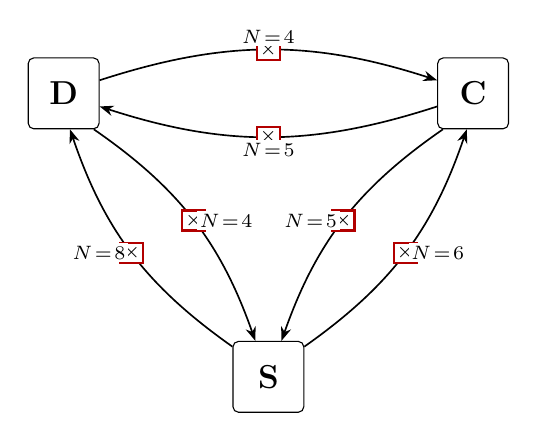
\begin{tikzpicture}[
    capability/.style={draw, rectangle, rounded corners=2pt, minimum size=9mm, font=\large\bfseries},
    arr/.style={-{Stealth[length=5pt]}, semithick},
    cross/.style={fill=white, draw=red!70!black, thick, inner sep=1pt, font=\scriptsize\bfseries},
    lbl/.style={font=\scriptsize, fill=white, inner sep=1pt},
  ]
  % Equilateral triangle, S at bottom center
  \node[capability] (S) at (0, 0) {S};
  \node[capability] (D) at (-2.6, 3.6) {D};
  \node[capability] (C) at ( 2.6, 3.6) {C};

  % D <-> C (top edge): upper arc and lower arc
  \draw[arr] (D.20) to[bend left=18] coordinate[midway] (DC) (C.160);
  \node[cross] at (DC) {$\times$};
  \node[lbl, above=1pt of DC] {$N\!=\!4$};

  \draw[arr] (C.200) to[bend left=18] coordinate[midway] (CD) (D.-20);
  \node[cross] at (CD) {$\times$};
  \node[lbl, below=1pt of CD] {$N\!=\!5$};

  % D <-> S (left edge): both bend left — outer arc goes left, inner goes right
  \draw[arr] (S.140) to[bend left=18] coordinate[midway] (SD) (D.280);
  \node[cross] at (SD) {$\times$};
  \node[lbl, left=1pt of SD] {$N\!=\!8$};

  \draw[arr] (D.310) to[bend left=18] coordinate[midway] (DS) (S.110);
  \node[cross] at (DS) {$\times$};
  \node[lbl, right=1pt of DS] {$N\!=\!4$};

  % C <-> S (right edge): mirror of left — both bend right
  \draw[arr] (S.40) to[bend right=18] coordinate[midway] (SC) (C.260);
  \node[cross] at (SC) {$\times$};
  \node[lbl, right=1pt of SC] {$N\!=\!6$};

  \draw[arr] (C.230) to[bend right=18] coordinate[midway] (CS) (S.70);
  \node[cross] at (CS) {$\times$};
  \node[lbl, left=1pt of CS] {$N\!=\!5$};
\end{tikzpicture}
\caption{Full independence structure. All six pairwise non-implications are proved by Lean-verified finite counterexamples at the indicated sizes. No capability implies any other.}
\label{fig:independence}
\end{figure}

\begin{theorem}[Full Independence]
\label{thm:independence}
No capability implies any other. Specifically, all six pairwise non-implications hold:
\begin{enumerate}
  \item $S \not\Rightarrow D$: An extensional 2-pointed magma of size $8$ satisfying S contains a classifier element but fails the global dichotomy condition.
  \item $S \not\Rightarrow C$: An extensional 2-pointed magma of size $6$ satisfying S has 4 core elements (enough for $\ICP$ to be non-vacuous) but no triple satisfies the $\ICP$.
  \item $D \not\Rightarrow C$: An extensional 2-pointed magma of size $4$ satisfying D has only 2 core elements, so $\ICP$ is vacuously unsatisfiable (pigeonhole).
  \item $C \not\Rightarrow D$: An extensional 2-pointed magma of size $5$ satisfies $\ICP$ but violates the classifier dichotomy. This is tight: $\ICP$ requires $N \geq 5$.
  \item $D \not\Rightarrow S$: An extensional 2-pointed magma of size $4$ satisfies the classifier dichotomy but admits no retraction pair. This is tight: D requires $N \geq 4$.
  \item $C \not\Rightarrow S$: An extensional 2-pointed magma of size $5$ satisfies $\ICP$ but admits no retraction pair. This is tight: $\ICP$ requires $N \geq 5$.
\end{enumerate}
\end{theorem}

\begin{proof}
Each direction is proved by exhibiting a concrete Cayley table and verifying the claimed properties by \texttt{native\_decide} (or \texttt{decide} for $N \leq 8$). The tables are:

\paragraph{$S \not\Rightarrow D$ ($N\!=\!8$).}
An $8 \times 8$ Cayley table (Appendix~\ref{app:tables}) defining an $\FRM$ with $s = 2$, $r = 3$. Element~4 is a classifier, but element~5's row on core is $(6, 2, 1, 1, 1, 1)$, mixing absorber and non-absorber outputs, violating the dichotomy. SAT confirms the non-implication is achievable as early as $N\!=\!3$, but vacuously: with only 1 core element, the dichotomy cannot be formulated (it requires both a classifier and a non-classifier). The $N\!=\!8$ witness is the smallest with enough core structure for D to be non-vacuously falsifiable. Lean file: \texttt{Countermodel.lean}.

\paragraph{$S \not\Rightarrow C$ ($N\!=\!6$, structural).}
A $6 \times 6$ Cayley table (Appendix~\ref{app:tables}) defining an extensional 2-pointed magma with a retraction pair ($s = r = 2$, an involution on core) but no $\ICP$. The core has 4 elements, more than the 3 pairwise distinct witnesses $\ICP$ requires, yet no triple satisfies the $\ICP$. As with $S \not\Rightarrow D$, the non-implication is vacuously achievable at $N\!=\!3$ (only 1 core element), but the $N\!=\!6$ witness is the smallest where $\ICP$ failure is structural rather than dimensional. Lean file: \texttt{E2PM.lean}, theorem \texttt{s\_not\_\allowbreak implies\_\allowbreak icp\_\allowbreak structural}.

\paragraph{$D \not\Rightarrow C$ ($N\!=\!4$, tight).}
The minimal S+D model at $N\!=\!4$ (\texttt{kripke4} in Appendix~\ref{app:tables}) has only 2 core elements. $\ICP$ requires 3 pairwise distinct non-absorbers, so it is vacuously unsatisfiable. Lean file: \texttt{ICP.lean}, theorem \texttt{kripke4\_no\_icp}. The $N\!=\!10$ D+S model in \texttt{Countermodels10.lean} complements this: it has 8 core elements (more than enough for $\ICP$ to be non-vacuous), yet no triple satisfies $\ICP$. The formal non-implication holds at $N\!=\!4$; the $N\!=\!10$ witness shows it persists even when C has room to exist.

\paragraph{$C \not\Rightarrow D$ ($N\!=\!5$, tight).}
A $5 \times 5$ Cayley table satisfying $\ICP$ but with no classifier: all three core elements map core to core (no element produces only absorber-valued outputs on core). The bound is tight: $\ICP$ requires $N \geq 5$. Lean file: \texttt{E2PM.lean}, theorem \texttt{h\_not\_implies\_d\_tight}.

\paragraph{$D \not\Rightarrow S$ ($N\!=\!4$, tight).}
A $4 \times 4$ Cayley table with the classifier dichotomy (classifier at index~2, non-classifier at index~3) but no retraction pair among the 4 possible assignments from core. The bound is tight: D requires $N \geq 4$. Lean file: \texttt{E2PM.lean}, theorem \texttt{d\_not\_implies\_s\_tight}.

\paragraph{$C \not\Rightarrow S$ ($N\!=\!5$, tight).}
A $5 \times 5$ Cayley table satisfying $\ICP$ but admitting no retraction pair. The bound is tight: $\ICP$ requires $N \geq 5$. Lean file: \texttt{E2PM.lean}, theorem \texttt{h\_not\_implies\_s\_tight}.

All tables are generated by Z3 SAT solver and independently verified. The Cayley tables are frozen in the repository for reproducibility.
\end{proof}

\paragraph{Methodology and minimality.}
Each counterexample was found by encoding the relevant capability axioms (and the negation of the target capability) as a SAT problem over an $n \times n$ Cayley table, then solving with Z3, incrementing $n$ from 3 upward. Once found, each table was frozen and independently verified in Lean. Four of six directions have provably tight bounds: D$\not\Rightarrow$S and D$\not\Rightarrow$C are tight at $N\!=\!4$ (the minimum where D is non-vacuous, resp.\ where $\ICP$ is dimensionally impossible); C$\not\Rightarrow$S and C$\not\Rightarrow$D are tight at $N\!=\!5$ (the minimum where $\ICP$ can be stated). The remaining two (S$\not\Rightarrow$D at $N\!=\!8$, S$\not\Rightarrow$C at $N\!=\!6$) are the smallest non-vacuous witnesses found. The SAT search was exhaustive: all smaller sizes returned UNSAT for every role assignment tested. Whether different role assignments or overlapping encodings could yield tighter witnesses is open.

\paragraph{Scaling.}
The independence is not a small-size artifact. For the coexistence direction, S+D+C is realized at every $N \geq 5$ by an explicit construction (Theorem~\ref{thm:scaling-witness}), so existence at all sufficiently large sizes is no longer empirical. For the six non-implication directions, we rely on SAT search: it confirms that all six are satisfiable at every size from their respective minima through $N\!=\!15$ (the solver limit), and no size was found where any direction becomes UNSAT. Whether each non-implication holds at all $n \geq $ its minimum (i.e.\ a witness exists at size $n$ for every $n$) remains a conjecture supported by this data, pending a constructive scaling argument analogous to Theorem~\ref{thm:scaling-witness}.

\paragraph{Interpretation.}
The independence result shows that S, D, and C are genuinely three things, not one. An algebra can encode and decode without classifying (S without D). An algebra can classify without encoding (D without S). An algebra can internally compose without classifying or encoding (C without S or D). No capability algebraically forces any other. In particular, the $C \not\Rightarrow D$ direction shows that an algebra can internalize a non-trivial composition pattern without satisfying the classifier dichotomy: internal composition does not force organizational separation.

\subsection{Joint irredundance: the Boolean cube}
\label{sec:boolean-cube}

Pairwise independence shows no capability implies any other. A stronger form of irredundance asks whether some capability is a \emph{Boolean function} of the other two: if $S$ were equivalent to $D \land \neg C$, say, the triple $(S, D, C)$ would collapse to the pair $(D, C)$. We rule this out by exhibiting a witness in each of the eight cells of the $(S, D, C)$ Boolean cube.

\begin{theorem}[Joint irredundance]
\label{thm:cube}
Each of the eight Boolean combinations of $(S, D, C)$ is realized by a Lean-verified finite extensional 2-pointed magma.
\end{theorem}

\begin{center}
\small
\begin{tabular}{clcl}
\textbf{Cell} & \textbf{Profile} & \textbf{N} & \textbf{Witness} \\
\hline
1 & $S \land D \land C$             & 5  & \texttt{witness5} \\
2 & $S \land D \land \neg C$        & 4  & \texttt{kripke4} \\
3 & $S \land \neg D \land C$        & 10 & \texttt{hNotD} \\
4 & $S \land \neg D \land \neg C$   & 3  & \texttt{frm3} (new) \\
5 & $\neg S \land D \land C$        & 5  & \texttt{cell5} (new) \\
6 & $\neg S \land D \land \neg C$   & 4  & \texttt{dNoS4} \\
7 & $\neg S \land \neg D \land C$   & 5  & \texttt{hNoD5} \\
8 & $\neg S \land \neg D \land \neg C$ & 3 & \texttt{cell8} (new) \\
\end{tabular}
\end{center}

Five cells are populated by witnesses that already appear in the pairwise-independence proof, after adding the missing capability annotations. Three required fresh constructions: cell~4 and cell~8 are minimal ($N\!=\!3$) FRM and E2PM witnessing ``S alone'' and ``no capability'' respectively; cell~5 (D and C without S) is the cube's most structurally constrained corner, an $N\!=\!5$ magma with two classifiers, one core-preserving non-classifier serving as the ICP's $b$, and no retraction pair. All verifications are machine-checked by \texttt{decide} or \texttt{native\_decide} in \texttt{BooleanCube.lean}.

The cell sizes reveal an asymmetry: every cell containing C requires $N \geq 5$, while cells with only S and/or D are realized at $N = 3$ or $4$. C carries strictly more structural weight than S or D, consistent with the row-scarcity argument in Section~\ref{sec:discussion}: ICP's factorization demand $a \dotop x = c \dotop (b \dotop x)$ constrains three rows simultaneously and requires three pairwise-distinct core elements, which S and D do not.

\paragraph{Consequence.}
If any capability were Boolean-equivalent to a combination of the other two, some cell would be empty. All cells are inhabited: no reduction of three predicates to two exists. S, D, and C therefore carry mutually irreducible information — jointly irredundant, not merely pairwise independent.

% ══════════════════════════════════════════════════════════════
\section{Coexistence}
\label{sec:bound}
% ══════════════════════════════════════════════════════════════

\begin{theorem}[No ICP at $N\!=\!4$]
\label{thm:no-icp-4}
No extensional 2-pointed magma of size $4$ satisfies the $\ICP$. The core $\{2,3\}$ has only 2 elements, but $\ICP$ requires 3 pairwise distinct non-absorbers. Lean: \texttt{Witness5.lean}, \texttt{no\_icp\_at\_4}.
\end{theorem}

\begin{theorem}[Coexistence Witness]
\label{thm:bound}
The three capabilities S, D, and C are simultaneously satisfiable. A Lean-verified witness exists at $N\!=\!5$, which is optimal by Theorem~\ref{thm:no-icp-4}.
\end{theorem}

\begin{proof}
A concrete $5 \times 5$ Cayley table is exhibited with $s\!=\!r\!=\!2$ (identity on core), classifiers $\tau \in \{3,4\}$, and $\ICP$ witnessed by $a\!=\!3, b\!=\!2, c\!=\!4$. The retraction pair collapses to a single element ($s\!=\!r$) which doubles as the $\ICP$'s core-preserving map; since $b$ is the identity, the factorization $a \cdot x = c \cdot (b \cdot x)$ reduces to $a \cdot x = c \cdot x$ on core, yielding two classifiers that agree on core but distinguished by their absorber columns. The lower bound is pigeonhole: at $N\!=\!4$, the core $\{2,3\}$ has only 2 elements, but $\ICP$ requires 3 pairwise distinct non-absorbers (\texttt{no\_icp\_at\_4}). Lean file: \texttt{Witness5.lean}, theorem \texttt{sdh\_witness\_5}. A $6 \times 6$ witness with $s \neq r$ is also verified (\texttt{Witness6.lean}).
\end{proof}

\begin{theorem}[Scaling: S+D+C exists at all $N \geq 5$]
\label{thm:scaling-witness}
For every integer $N \geq 5$, there exists an extensional 2-pointed magma on $\Fin(N)$ satisfying S, D, and C. Lean: \texttt{WitnessAllN.lean}, theorem \texttt{sdh\_witness\_all\_N}.
\end{theorem}

\begin{proof}[Proof (constructive)]
For $N \geq 5$, define $T_N : \Fin(N) \times \Fin(N) \to \Fin(N)$ by:
\begin{itemize}
  \item $T_N(0, x) = 0$ for all $x$.
  \item $T_N(1, x) = 1$ for all $x$.
  \item $T_N(2, x) = x$ for all $x$.
  \item $T_N(3, x) = 1$ if $x \in \{3, 4\}$, else $T_N(3, x) = 0$.
  \item $T_N(4, x) = 1$ if $x \in \{1, 3, 4\}$, else $T_N(4, x) = 0$.
  \item For $k \in \{5, \ldots, N-1\}$: $T_N(k, 2) = k$, $T_N(k, k) = 2$, and $T_N(k, x) = x$ for all $x \notin \{2, k\}$.
\end{itemize}

\emph{E2PM axioms.} Rows $0$ and $1$ are constant absorbers. For $k \in \{2, 3, 4\}$ row $k$ takes at least two values, so no row beyond rows $0, 1$ is constant. Extensionality: rows $0, 1$ differ from each other and from all higher rows at column $0$ (row $0$ has $0$, row $1$ has $1$, row $k \geq 2$ has $0$). Row $2$ differs from rows $3, 4$ at column $2$ (row $2$ has $2$, rows $3, 4$ have $0$). Rows $3$ and $4$ differ at column $1$. For $k, k' \in \{5, \ldots, N-1\}$ with $k \neq k'$: rows $k$ and $k'$ differ at column $k$ (row $k$ has $2$, row $k'$ has $k$).

\emph{S.} Take $s = r = 2$. Anchoring $T_N(2, 0) = 0$ holds. The retraction equations $T_N(2, T_N(2, x)) = T_N(2, x) = x$ on $\core(S)$ hold trivially since row $2$ is identity.

\emph{D.} Rows $3$ and $4$ have values in $\{0, 1\}$ everywhere, so they are full classifiers. Rows $2$ and $k$ for $k \geq 5$ map $\core(S)$ into $\core(S)$ (verified by inspection), so they are non-classifiers. The dichotomy holds. Take $\tau = 3$ as the full classifier; the non-classifier $2$ exists.

\emph{C.} The triple $(3, 2, 4)$ is an H-triple: the three indices are pairwise distinct in $\core(S)$; row $2$ is core-preserving; for $x \in \core(S)$, $T_N(3, x) = T_N(4, T_N(2, x))$ holds because row $2$ is identity, so $T_N(3, x) = T_N(4, T_N(2, x)) = T_N(4, x)$ reduces to row equality on core, which holds by direct comparison (both rows are constant $0$ on $\core \setminus \{3, 4\}$ and constant $1$ on $\{3, 4\}$); $T_N(3, \cdot)|_{\core(S)}$ takes both values $0$ and $1$ (at $x = 2$ and $x = 3$ respectively), so non-triviality holds.
\end{proof}

\begin{proposition}[Separated-Role Witness]
\label{thm:separated}
There is a witness at $N\!=\!10$ in which the principal S+D+C roles (2 absorbers, 2 retraction pair, 1 classifier, 3 $\ICP$ witnesses) occupy 8 distinct elements.
\end{proposition}

\begin{proof}
A concrete $10 \times 10$ Cayley table (Appendix~\ref{app:tables}) satisfies all three capabilities with distinct role assignments. Lean file: \texttt{Witness10.lean}. A witness with $s \neq r$ (non-degenerate retraction) is exhibited at $N\!=\!6$ (Appendix~\ref{app:tables}).
\end{proof}

\paragraph{Minimum cardinality.}
$N\!=\!5$ is the optimal minimum for S+D+C coexistence (Lean-verified; \texttt{Witness5.lean}). The witness uses $s = r$ (identity on core), two classifiers, and one non-classifier: the retraction pair member doubles as the ICP's core-preserving element. At $N\!=\!4$ the core has only 2 elements but ICP requires 3 pairwise distinct non-absorbers, so $N\!=\!4$ is impossible (\texttt{no\_icp\_at\_4}).

The $N\!=\!5$ witness reveals how thin the three properties can become simultaneously. The retraction pair is the identity on core ($s = r$, no actual encoding work), and the ICP factorization $a \dotop x = c \dotop (b \dotop x)$ collapses to $a \dotop x = c \dotop x$ (row equality on core between two classifiers differing only on absorber columns). The three capabilities are formally present but barely interacting. The $N\!=\!6$ witness with $s \neq r$ (\texttt{Witness6.lean}) is the more informative example: the retraction pair does genuine encoding, the ICP factorization is non-degenerate, and the roles do not trivially overlap. We retain the general definitions (allowing $s = r$) since the algebraic results (independence, injectivity, no-associativity) hold regardless.

% ══════════════════════════════════════════════════════════════
\section{Related Work}
\label{sec:related}
% ══════════════════════════════════════════════════════════════

\paragraph{Partial and total combinatory algebras.}
PCAs~\cite{vanoosten08,longley15} and TCAs~\cite{bethke88} provide the standard algebraic framework for realizability and computability. PCA theory has a rich structural theory: morphisms between PCAs, the lattice of PCA quotients, and totalizability~\cite{bethke96} all involve detailed analysis of the application operation. PCA theory does study which elements realize which functions. However, this analysis concerns representability and inter-PCA relationships, not the \emph{partition} of elements into behavioral types by their row structure. This question requires a finite total operation table to formulate; it does not arise in the PCA/TCA setting, where application is partial or the carrier is infinite. Bethke and Klop~\cite{bethke96} proved that some PCAs cannot be extended to total ones, a structural result about the relationship between partiality and totality. The K-infinity theorem (our Theorem~\ref{thm:k-infinity}) shows that nontrivial S+K algebras must be infinite, explaining why finite algebras fall outside this framework and why our setting requires a different combinator basis.

\paragraph{Turing categories.}
Cockett and Hofstra~\cite{cockett08} define a Turing category as a cartesian restriction category with a Turing object~$A$ and a Turing morphism $\bullet : A \times A \to A$ that universally simulates all morphisms in the category. The Structure Theorem establishes that PCAs and Turing categories are two views of the same concept. Turing objects have cardinality ``one or infinite''~\cite{cockett08}, ruling out nontrivial finite Turing objects. The Turing morphism is described as ``the heart of the whole structure'' but its algebraic properties (row structure, element classification, associativity constraints) are not studied. Where Turing categories distribute computational roles across distinct objects (programs, data, evaluators), our finite algebras develop the same roles internally as emergent behavioral regions within a single carrier set: absorbers encode failure, classifiers provide absorber-valued judgment, and the retraction pair provides encoding.

\paragraph{Self-interpretation.}
Mogensen~\cite{mogensen92} constructs self-interpreters for the $\lambda$-calculus. Brown and Palsberg~\cite{brown16} show that self-interpretation is possible in strongly-normalizing typed languages, contradicting earlier impossibility results. These works study self-interpretation (our S) but do not address the independence of S from D or C.

\paragraph{Independence in finite algebra.}
Independence and non-implication results between equational properties have a long history in universal algebra, from Birkhoff's characterization of equational classes~\cite{burris81} to Mal'cev conditions characterizing implications between properties of varieties. Our results operate at a different level: we separate \emph{operational} properties (retraction pairs, classifier partitions, factorizations in the left-regular representation) rather than equational identities, and our base class, the finite extensional 2-pointed magmas, is not a variety in the Birkhoff sense (extensionality is a quasi-identity, not an equation). To our knowledge, the pairwise independence of retraction pairs, classifier dichotomies, and factorization properties in finite magmas has not been previously established. The SAT-find-then-Lean-verify methodology is related to the use of automated tools such as Mace4~\cite{mccune10} for counterexample search in algebra, though we use Z3 for constraint solving and Lean~4 for independent formal verification.

\paragraph{Finite model theory and machine-checked proofs.}
Independence results via finite counterexamples are standard in finite model theory~\cite{libkin04}. Each Cayley table is frozen in the Lean source and verified by the kernel, eliminating transcription errors. The sizes involved ($N\!=\!5$ through $N\!=\!10$) are small enough for \texttt{decide}/\texttt{native\_decide} but large enough that hand-verification of all conditions would be error-prone. The universal algebraic theorems (no-associativity, decomposition invariance, ICP equivalence) are proved by pure equational reasoning without \texttt{decide}, and hold for all finite sizes.

\paragraph{Cellular automata and applicative calculus.}
The structures studied here sit at an intersection of two computational-substrate traditions that have otherwise remained separate. Cellular automata (Rule 110, Conway's Game of Life, and the broader tradition) establish universality from a finite local rule by iterated unfolding; the rule itself is small and fixed, while computation emerges from temporal-spatial extent. Applicative calculi (combinatory logic, the $\lambda$-calculus) take the binary application operation as primitive and use extensionality to individuate functions by behavior. Finite extensional 2-pointed magmas inherit the finite-local-rule nature of cellular automata (the Cayley table is the rule; computation unfolds as a term tree) together with the applicative-and-extensional structure of combinatory calculi (the operation is $a \dotop b$, asymmetric between operator and operand, with rows individuating elements). They differ from each tradition in specific ways: from cellular automata, they drop the spatial grid, replacing it with term-tree unfolding; from combinatory calculi, they drop abstraction, fixing the entire function inventory as the finite carrier. Neither tradition has systematically studied the resulting hybrid --- finite applicative substrates with extensional individuation --- and in particular the capability-decomposition questions (what can be internalized as element behavior modulo the operation?) answered by this paper do not arise naturally in either parent.

% ══════════════════════════════════════════════════════════════
\section{Discussion}
\label{sec:discussion}
% ══════════════════════════════════════════════════════════════

\paragraph{The classifier dichotomy is organizational.}
D organizes elements into coherent categories: classifiers that test and non-classifiers that transform. The $C \not\Rightarrow D$ result shows that an algebra can internalize composition without this organization. D contributes semantic structure rather than compositional behavior.

\paragraph{Why magmas?}
Magmas are not a limitation but a natural choice, for two independent reasons. First, the K-infinity theorem (Theorem~\ref{thm:k-infinity}) shows that nontrivial combinatory algebras with $\mathbf{s}$ and $\mathbf{k}$ must be infinite: the $\mathbf{k}$ combinator is a non-surjective injection on any finite set with $\geq 2$ elements. Finite internal dichotomy requires a different combinator basis, one without a K-like projector, and our extensional 2-pointed magmas provide exactly this. Second, Theorem~\ref{thm:no-assoc} shows that associativity forces any classifier to have a constant row, collapsing it to an absorber. Combined with the no-right-identity result (Theorem~\ref{thm:no-rid}), this independently rules out the entire classical algebraic hierarchy: no semigroup, monoid, group, or ring can support the classifier dichotomy alongside a retraction pair. Self-description lives outside both the PCA/TCA framework (by cardinality) and the classical algebraic hierarchy (by associativity). This connects to the broader observation that reflective systems are inherently non-associative: $\lambda$-calculus application is non-associative ($(f\,g)\,x \neq f\,(g\,x)$ in general). The no-associativity theorem shows this is algebraically forced, not a design accident.

\paragraph{Finiteness is essential, not merely technical.}
Finiteness plays two roles in this paper. Technically, it makes \texttt{decide} and \texttt{native\_decide} applicable to the counterexamples. Substantively, it underwrites the K-infinity obstruction (Theorem~\ref{thm:k-infinity}) and the row-scarcity argument behind the independence of D and C (below): the structures studied here are those whose internal dichotomy is of a completed totality, with a bounded supply of rows. On infinite carriers that constraint dissolves and the independence need not transfer; extending it beyond the finite setting is a separate question about a structurally different phenomenon.

\paragraph{The role of extensionality.}
Extensionality (distinct elements have distinct rows) is load-bearing throughout. Without it, the no-associativity proof fails: Step~4 derives $\tau = v$ from identical rows. Without it, any constant-row element trivially satisfies both classifier and non-classifier conditions, making the three-category decomposition degenerate. Extensionality is not merely a convenience but the condition that makes element-level classification meaningful. An element's identity \emph{is} its row in the Cayley table; extensionality formalizes this.

\paragraph{Why these three properties?}
Extensionality identifies each element with its row in the Cayley table. The elements of a finite extensional 2-pointed magma are therefore a family of typed maps $\{L_a^{\core} : \core \to \core \cup Z\}$, one per element, with the absorber maps $L_{z_1}, L_{z_2}$ being constant. S, D, and C correspond to the three fundamental structural questions about such a family:
\begin{itemize}
  \item \emph{Splitting} (S): does the identity on core split through the family? That is, do some $L_s, L_r$ satisfy $L_r \circ L_s = \mathrm{id}_{\core}$? This is a section-retraction pair~\cite{maclane71}.
  \item \emph{Codomain purity} (D): does each map hit $\core$ or $Z$, never both? This is the unique coarsest non-trivial isomorphism-invariant partition of core (Corollary~\ref{cor:canonicity}).
  \item \emph{Factorization} (C): does the family contain a non-trivial composition, $L_a = L_c \circ L_b$ with $L_b$ core-preserving and $L_a$ non-constant? This is the weakest factorization condition that is not vacuously satisfiable: weakening either the pairwise-distinctness or the non-triviality requirement makes every retraction-equipped magma satisfy it trivially (Lean-verified separations in \texttt{ICP.lean}).
\end{itemize}
Each property is minimal in its own sense. S is the standard notion of splitting. D is the coarsest invariant partition. C is the weakest non-degenerate factorization. The independence and joint-irredundance results (Theorems~\ref{thm:independence},~\ref{thm:cube}) confirm these are three questions jointly irredundant, not reducible to two. The precise categorical status of D and C is discussed further in the categorical connections paragraph below; whether either corresponds to a known universal property remains open.

\paragraph{Minimality of the kernel.}
Theorem~\ref{thm:cube} establishes that no capability is a Boolean function of the other two, so $(S, D, C)$ cannot be compressed to a pair under any Boolean reduction. A stronger claim --- that S, D, and C constitute a \emph{canonical} kernel in the sense that every ``natural'' operational axiom on E2PM is either vacuous, equivalent to one of $S, D, C$, implied by one of them, or captured by their Boolean combination --- is false, and we record this honestly. A Z3 canonicality probe (\texttt{scripts/canonicality/probe\_axioms.py}) tested thirteen candidate operational axioms on E2PM at $N = 5$ and $N = 6$, running all eight pairwise directional implication queries (\mbox{$E2PM + A_k + \neg X$} and \mbox{$E2PM + X + \neg A_k$} for $X \in \{S, D, C\}$) per axiom. Ten of the thirteen are pairwise independent of $S, D, C$ in both directions at both sizes, including first-instinct properties such as ``$\exists\, y \in \core$ with $y \dotop y = y$'' (idempotent element), ``$\exists\, y \in \core$ with $y \dotop (y \dotop x) = x$ on core'' (self-involution), and ``$\exists\, y_1 \neq y_2 \in \core$ with $y_1 \dotop y_2 = y_2 \dotop y_1$'' (commutative pair). Three candidates cleanly collapse: $S$ implies the one-sided retraction condition and the left-cancellation property; $D$ and $C$ both imply $P$ (\emph{internal preservation}, the common substructure identified in the paragraph ``A common substructure: core-preserving rows'' following Proposition~\ref{prop:N6-h-triples}).

The picture is one of \emph{a rich internalization landscape}, not a minimal kernel. The probe's finding --- that many natural operational properties are independent of $S, D, C$ --- is not a deficiency but direct evidence that $(A, \dotop)$ is a structurally fertile substrate on which many different services can be separately internalized. What distinguishes S, D, and C is not that they exhaust this landscape --- they do not --- but that each names a specific structural phenomenon the paper proves something concrete about: the retraction's role lock-in at $N\!=\!5$ and its phase transition at $N \geq 6$ (Theorem~\ref{thm:N5-structure}, Proposition~\ref{prop:N6-nonrigid}); the functorial invariance and three-category decomposition induced by D (Corollary~\ref{cor:canonicity}, Theorem~\ref{thm:cap-invariance}); and the ICP / Compose+Inert equivalence for C (Theorem~\ref{thm:icp-equiv}). Minimality in the strong operational sense fails; minimality in the Boolean sense (Theorem~\ref{thm:cube}) holds; and the smaller positive finding --- that $P$ (internal preservation) is a common substructure of D and C, with D decomposing cleanly through it --- emerges directly from the same probe.

\paragraph{Categorical connections and their limits.}
Several constructions in this paper have natural categorical readings. The core $\core(S)$ is a retract of the carrier via $(s, r)$, in the standard sense of~\cite{maclane71}. The three-category decomposition defines a functor from the category $\mathbf{E2PM}$ (extensional 2-pointed magmas with absorber-preserving homomorphisms) to the category of three-block set partitions: Theorems~\ref{thm:functoriality} and~\ref{thm:cap-invariance} establish that both the decomposition and the three capabilities are preserved by morphisms. The classifier dichotomy is a codomain-purity condition on the family of left-multiplication maps $\{L_a^{\core} : \core \to \core \cup Z\}$, partitioning them by image type.

The categorical analogy breaks down at composition. The left-multiplication maps $L_a^{\core}$ are not closed under composition: $L_a \circ L_b$ need not equal $L_c$ for any element $c$. For instance, in the $N\!=\!5$ coexistence witness, $L_2 \circ L_3$ on core gives $(0, 2, 0)$, which is not the core row of any element. This means the row family does not form a transformation monoid, and standard categorical constructions (internal hom, enrichment, Turing morphism) cannot be stated internally. The no-associativity theorem (Theorem~\ref{thm:no-assoc}) predicts this failure: associativity of the magma operation would be a prerequisite for the left-multiplication maps to form a monoid, and the theorem shows associativity is incompatible with the S+D structure. The composition-closure failure is not a gap in the formalization but a consequence of the same obstruction that motivates the setting.

\paragraph{Why the independence holds.}
The independence of D and C reflects incompatible row constraints under finiteness. A classifier's row is fully committed to absorber values on core: every core input maps to $z_1$ or $z_2$. An ICP witness $a$ requires $a \dotop x = c \dotop (b \dotop x)$ with at least two distinct values on core, so its row must be non-trivially structured. These demands are incompatible for any single element, so different elements must carry these roles. The independence holds because finiteness limits the total supply of elements and constrains which row patterns can coexist under extensionality. The $C \not\Rightarrow D$ direction has the same character: an ICP triple $(a, b, c)$ constrains three rows to satisfy a factorization equation, but this imposes no absorber-output condition on any fourth element.

\paragraph{The infinite boundary.}
In infinite carriers where the set of left-multiplication maps is unconstrained, such as the full function space over a countable set, the row-scarcity constraint dissolves. The carrier is large enough to accommodate elements with arbitrary row patterns, and the tension between classifier rows and factorization rows need not arise. Whether the independence survives in specific infinite algebraic settings is open. This is an observation about resource limitations, not a theorem about Turing completeness: the precise conditions under which the independence transfers require defining the relevant algebraic properties for infinite carriers, which is beyond this paper's scope.

\paragraph{S as a separate design choice.}
The independence of S from D and C plausibly extends beyond finite magmas. A faithful internal encoding, a section-retraction pair on the carrier, is a separate design choice from classification or composition. Mogensen's self-interpreter for the $\lambda$-calculus~\cite{mogensen92} requires an explicit quoting convention; without it, the calculus is computationally universal but lacks internal splitting. This suggests that the S independence is not an artifact of finiteness but reflects a genuine structural distinction between having computational capabilities and having a faithful encoding of one's own elements as data.

\paragraph{Scope and limitations.}
Whether the three-capability separation appears in other settings ($\lambda$-calculus, typed systems, infinite algebras) is the primary open question. Theorem~\ref{thm:no-assoc} constrains the target: any such translation must work without associativity or identity. Each capability admits multiple axiom forms; the independence result holds for all variants. The independence also implies that any system combining all three capabilities must introduce additional axioms beyond S, D, and C to connect them; the nature of these connecting axioms is a natural direction for further work.

% ══════════════════════════════════════════════════════════════
\section{Conclusion}
% ══════════════════════════════════════════════════════════════

Four obstructions --- K-infinity, no-associativity, asymmetry, and single-absorber collapse --- jointly narrow the candidate class of finite magmas that can carry the operational capabilities of splitting, dichotomy, and composition down to the setting of this paper: finite, non-associative, non-commutative, extensional 2-pointed magmas. Within it, we have identified three natural algebraic properties, internal splitting~(S), the classifier dichotomy~(D), and the Internal Composition Property~(C), and proved they are pairwise independent. The six non-implications are machine-checked in Lean~4. Joint irredundance strengthens this: all eight Boolean combinations of $(S, D, C)$ are realized (Theorem~\ref{thm:cube}), so no capability is a Boolean function of the other two. The optimal coexistence witness has $N\!=\!5$ (Theorem~\ref{thm:bound}). The three-category decomposition induced by D is a functorial invariant (Theorem~\ref{thm:functoriality}); the principal coexistence witnesses are role-rigid (Proposition~\ref{prop:witness-rigid}); at $N\!=\!5$ a structure theorem pins retraction, classifier, and C-triple onto the three core slots and rules out strong S altogether (Theorem~\ref{thm:N5-structure}), while at $N \geq 6$ strong S returns and rigidity fails (Proposition~\ref{prop:N6-nonrigid}); and the ICP is logically equivalent to Compose+Inert (Theorem~\ref{thm:icp-equiv}). Lean-formalized results --- independence counterexamples, joint-irredundance witnesses, decomposition invariance, the ICP equivalence, the all-$N$ scaling witness (Theorem~\ref{thm:scaling-witness}), H-triple type-coherence (Theorem~\ref{thm:h-triple-coherence}), and the $N\!=\!5$ structure theorem (Theorem~\ref{thm:N5-structure}) --- compile with zero \texttt{sorry}. The remaining universal-$N$ algebraic results of Section~\ref{sec:universal} not yet transcribed to Lean (most notably the P-witness identity of Theorem~\ref{thm:p-witness-identity} and the classifier-count bound of Theorem~\ref{thm:classifier-count-bound}) are proved by hand and supported by Z3 UNSAT certificates.

\paragraph{Open problems.}
\begin{enumerate}
  \item \emph{Cross-formalism universality}: Does the three-capability separation appear in the $\lambda$-calculus, typed settings, or infinite algebras? The no-associativity obstruction (Theorem~\ref{thm:no-assoc}) constrains the target setting.
  \item \emph{Categorical characterization of C}: The ICP is the weakest non-degenerate factorization property of the left-regular representation (weakening either pairwise-distinctness or non-triviality makes it vacuous). Is it equivalent to a standard universal property (e.g., existence of a partial internal hom)?
  \item \emph{Categorical characterization of D}: D is the unique coarsest non-trivial isomorphism-invariant partition of core (Corollary~\ref{cor:canonicity}), isolating the two-valued aspect of a subobject classifier without the universality aspect. The left-multiplication maps lack composition closure, precluding standard categorical formulations. Does D correspond to a known concept in non-associative categorical algebra, or does it constitute a new structural property?
  \item \emph{Rigidity propagation beyond $N\!=\!5$}: Theorem~\ref{thm:N5-structure} establishes a rigid role assignment at $N\!=\!5$ (and in particular rules out strong S), but rigidity fails at $N\!=\!6, 7, 8$ under strong S (Proposition~\ref{prop:N6-nonrigid}). Several natural single-axiom strengthenings (classifier-nontriviality on core, asymmetric anchoring of the section, anchor monotonicity, strict anchor asymmetry) were each tested and each Z3-satisfiable alongside a non-trivial automorphism at some $N \in \{6, 7, 8\}$ (scripts and witness JSONs under \texttt{scripts/}). Characterizing the minimum axiom system that uniformly forces role-rigidity at $N \geq 5$ --- and whether it admits a bounded finite specification --- is open.
\end{enumerate}

\paragraph{Artifact.}
All Lean files, counterexample tables, and SAT reproduction scripts are available at \url{https://github.com/stefanopalmieri/finite-magma-independence}.

% ══════════════════════════════════════════════════════════════
% References
% ══════════════════════════════════════════════════════════════

\begin{thebibliography}{20}

\bibitem{smith84}
Brian Cantwell Smith.
\newblock Reflection and semantics in {Lisp}.
\newblock In \emph{POPL}, pages 23--35, 1984.

\bibitem{mogensen92}
Torben Mogensen.
\newblock Efficient self-interpretation in lambda calculus.
\newblock \emph{Journal of Functional Programming}, 2(3):279--291, 1992.

\bibitem{brown16}
Matt Brown and Jens Palsberg.
\newblock Breaking through the normalization barrier: A self-interpreter for {F-omega}.
\newblock In \emph{POPL}, pages 5--17, 2016.

\bibitem{maclane71}
Saunders Mac~Lane.
\newblock \emph{Categories for the Working Mathematician}.
\newblock Springer, 1971.

\bibitem{johnstone02}
Peter~T. Johnstone.
\newblock \emph{Sketches of an Elephant: A Topos Theory Compendium}, vol.~1.
\newblock Oxford University Press, 2002.

\bibitem{libkin04}
Leonid Libkin.
\newblock \emph{Elements of Finite Model Theory}.
\newblock Springer, 2004.

\bibitem{burris81}
Stanley Burris and H.~P. Sankappanavar.
\newblock \emph{A Course in Universal Algebra}.
\newblock Springer, 1981.

\bibitem{scott72}
Dana Scott.
\newblock Continuous lattices.
\newblock In \emph{Toposes, Algebraic Geometry and Logic}, vol.~274 of \emph{Lecture Notes in Mathematics}, pages 97--136. Springer, 1972.

\bibitem{mccune10}
William McCune.
\newblock \emph{Prover9 and Mace4}.
\newblock \url{https://www.cs.unm.edu/~mccune/prover9/}, 2005--2010.

\bibitem{moura21}
Leonardo de~Moura and Sebastian Ullrich.
\newblock The {Lean}~4 theorem prover and programming language.
\newblock In \emph{CADE}, pages 625--635, 2021.

\bibitem{vanoosten08}
Jaap van~Oosten.
\newblock \emph{Realizability: An Introduction to its Categorical Side}.
\newblock Studies in Logic and the Foundations of Mathematics~152, Elsevier, 2008.

\bibitem{longley15}
John Longley and Dag Normann.
\newblock \emph{Higher-Order Computability}.
\newblock Theory and Applications of Computability, Springer, 2015.

\bibitem{bethke88}
Ingemarie Bethke.
\newblock \emph{Notes on Partial Combinatory Algebras}.
\newblock PhD thesis, Universiteit van Amsterdam, 1988.

\bibitem{bethke96}
Ingemarie Bethke and Jan~Willem Klop.
\newblock Collapsing partial combinatory algebras.
\newblock In \emph{Higher-Order Algebra, Logic, and Term Rewriting (HOA 1995)}, LNCS~1074, pages 16--48, Springer, 1996. \textsc{doi}: 10.1007/3-540-61254-8\_18.

\bibitem{cockett08}
J.~Robin~B. Cockett and Pieter Hofstra.
\newblock Introduction to {T}uring categories.
\newblock \emph{Annals of Pure and Applied Logic}, 156(2--3):183--209, 2008. \textsc{doi}: 10.1016/j.apal.2008.04.005.

\end{thebibliography}

% ══════════════════════════════════════════════════════════════
\appendix
% ══════════════════════════════════════════════════════════════

\section{Cayley Tables}
\label{app:tables}

All tables are extracted from the Lean source files and verified by \texttt{lake build}. Element $i$'s row is row~$i$; entry $(i,j)$ is $i \dotop j$.

\paragraph{$N\!=\!4$: Minimal S+D witness ($s = r$).}
Roles: $0 = z_1$, $1 = z_2$, $2 = \tau$, $3 = s = r$. \quad Lean: \texttt{CatKripkeWallMinimal.lean}, \texttt{kripke4}.

\medskip
{\small
\begin{tabular}{c|cccc}
$\dotop$ & 0 & 1 & 2 & 3 \\\hline
0 & 0 & 0 & 0 & 0 \\
1 & 1 & 1 & 1 & 1 \\
2 & 0 & 1 & 0 & 1 \\
3 & 0 & 0 & 2 & 3 \\
\end{tabular}}

\paragraph{$N\!=\!5$: Minimal S+D witness ($s \neq r$).}
Roles: $0 = z_1$, $1 = z_2$, $2 = s$, $3 = r$, $4 = \tau$. \quad Lean: \texttt{CatKripkeWallMinimal.lean}, \texttt{kripke5}.

\medskip
{\small
\begin{tabular}{c|ccccc}
$\dotop$ & 0 & 1 & 2 & 3 & 4 \\\hline
0 & 0 & 0 & 0 & 0 & 0 \\
1 & 1 & 1 & 1 & 1 & 1 \\
2 & 1 & 0 & 3 & 4 & 2 \\
3 & 0 & 2 & 4 & 2 & 3 \\
4 & 0 & 1 & 1 & 0 & 0 \\
\end{tabular}}

\paragraph{$N\!=\!5$: S+D+C Optimal Coexistence ($s = r$, minimal coexistence witness).}
Roles: $0 = z_1$, $1 = z_2$, $2 = s = r$ (identity on core, ICP $b$), $3 = \tau$ (classifier, ICP $a$), $4 = \tau_2$ (classifier, ICP $c$). \quad Lean: \texttt{Witness5.lean}.

\medskip
{\small
\begin{tabular}{c|ccccc}
$\dotop$ & 0 & 1 & 2 & 3 & 4 \\\hline
0 & 0 & 0 & 0 & 0 & 0 \\
1 & 1 & 1 & 1 & 1 & 1 \\
2 & 0 & 1 & 2 & 3 & 4 \\
3 & 0 & 0 & 0 & 1 & 1 \\
4 & 0 & 1 & 0 & 1 & 1 \\
\end{tabular}}

\paragraph{$N\!=\!6$: S+D+C Coexistence (role overlap).}
Roles: $0 = z_1$, $1 = z_2$, $2 = s$ (also ICP $a$), $3 = r$ (also ICP $b$), $4 = \tau$, $5 =$ ICP $c$. \quad Lean: \texttt{Witness6.lean}.

\medskip
{\small
\begin{tabular}{c|cccccc}
$\dotop$ & 0 & 1 & 2 & 3 & 4 & 5 \\\hline
0 & 0 & 0 & 0 & 0 & 0 & 0 \\
1 & 1 & 1 & 1 & 1 & 1 & 1 \\
2 & 3 & 3 & 4 & 2 & 5 & 3 \\
3 & 0 & 1 & 3 & 5 & 2 & 4 \\
4 & 0 & 0 & 1 & 0 & 1 & 1 \\
5 & 2 & 2 & 5 & 4 & 3 & 2 \\
\end{tabular}}

\paragraph{$N\!=\!8$: $S \not\Rightarrow D$ Counterexample.}
Roles: $0 = z_1$, $1 = z_2$, $2 = s$, $3 = r$, $4 =$ classifier, $5, 7 =$ mixed (violate dichotomy). \quad Lean: \texttt{Countermodel.lean}.

\medskip
{\small
\begin{tabular}{c|cccccccc}
$\dotop$ & 0 & 1 & 2 & 3 & 4 & 5 & 6 & 7 \\\hline
0 & 0 & 0 & 0 & 0 & 0 & 0 & 0 & 0 \\
1 & 1 & 1 & 1 & 1 & 1 & 1 & 1 & 1 \\
2 & 3 & 3 & 7 & 3 & 4 & 6 & 5 & 2 \\
3 & 0 & 1 & 7 & 3 & 4 & 6 & 5 & 2 \\
4 & 0 & 0 & 0 & 0 & 0 & 0 & 1 & 0 \\
5 & 6 & 2 & 6 & 2 & 1 & 1 & 1 & 1 \\
6 & 0 & 0 & 5 & 2 & 2 & 2 & 2 & 2 \\
7 & 2 & 2 & 2 & 1 & 2 & 2 & 6 & 3 \\
\end{tabular}}

\paragraph{$N\!=\!6$: $S \not\Rightarrow C$ Counterexample (structural).}
Roles: $0 = z_1$, $1 = z_2$, $2 = s = r$ (involution on core). Retraction pair holds; no triple satisfies $\ICP$ despite 4 core elements. \quad Lean: \texttt{E2PM.lean} (\texttt{sNoH6\_e2pm}).

\medskip
{\small
\begin{tabular}{c|cccccc}
$\dotop$ & 0 & 1 & 2 & 3 & 4 & 5 \\\hline
0 & 0 & 0 & 0 & 0 & 0 & 0 \\
1 & 1 & 1 & 1 & 1 & 1 & 1 \\
2 & 0 & 3 & 3 & 2 & 5 & 4 \\
3 & 2 & 4 & 5 & 5 & 1 & 4 \\
4 & 5 & 3 & 0 & 0 & 3 & 2 \\
5 & 4 & 2 & 2 & 2 & 2 & 2 \\
\end{tabular}}

\paragraph{$N\!=\!10$: $D \not\Rightarrow C$ Counterexample.}
Roles: $0 = z_1$, $1 = z_2$, $2 = s$, $3 = r$, $4 = \tau$. No triple satisfies $\ICP$. \quad Lean: \texttt{Countermodels10.lean} (\texttt{dNotH}), \texttt{ICP.lean} (\texttt{dNotH\_no\_icp}).

\medskip
{\footnotesize
\begin{tabular}{c|cccccccccc}
$\dotop$ & 0 & 1 & 2 & 3 & 4 & 5 & 6 & 7 & 8 & 9 \\\hline
0 & 0 & 0 & 0 & 0 & 0 & 0 & 0 & 0 & 0 & 0 \\
1 & 1 & 1 & 1 & 1 & 1 & 1 & 1 & 1 & 1 & 1 \\
2 & 3 & 3 & 2 & 3 & 4 & 5 & 6 & 7 & 9 & 8 \\
3 & 0 & 1 & 2 & 3 & 4 & 5 & 6 & 7 & 9 & 8 \\
4 & 0 & 0 & 1 & 1 & 1 & 1 & 1 & 1 & 1 & 1 \\
5 & 1 & 0 & 0 & 0 & 0 & 0 & 0 & 0 & 0 & 0 \\
6 & 2 & 3 & 9 & 9 & 9 & 9 & 9 & 9 & 9 & 8 \\
7 & 3 & 2 & 9 & 9 & 9 & 9 & 9 & 9 & 9 & 8 \\
8 & 1 & 0 & 1 & 0 & 1 & 1 & 1 & 1 & 0 & 0 \\
9 & 0 & 1 & 0 & 1 & 0 & 1 & 1 & 0 & 1 & 1 \\
\end{tabular}}

\paragraph{$N\!=\!10$: $C \not\Rightarrow D$ Counterexample.}
Roles: $0 = z_1$, $1 = z_2$, $2 = s$, $3 = r$, $4 = \tau$. $\ICP$ holds ($a\!=\!8, b\!=\!6, c\!=\!7$). Element~5 violates dichotomy. \quad Lean: \texttt{Countermodels10.lean} (\texttt{hNotD}).

\medskip
{\footnotesize
\begin{tabular}{c|cccccccccc}
$\dotop$ & 0 & 1 & 2 & 3 & 4 & 5 & 6 & 7 & 8 & 9 \\\hline
0 & 0 & 0 & 0 & 0 & 0 & 0 & 0 & 0 & 0 & 0 \\
1 & 1 & 1 & 1 & 1 & 1 & 1 & 1 & 1 & 1 & 1 \\
2 & 3 & 1 & 3 & 4 & 9 & 6 & 8 & 5 & 7 & 2 \\
3 & 0 & 1 & 9 & 2 & 3 & 7 & 5 & 8 & 6 & 4 \\
4 & 0 & 0 & 1 & 1 & 1 & 1 & 1 & 1 & 0 & 0 \\
5 & 0 & 0 & 2 & 0 & 0 & 0 & 0 & 0 & 3 & 1 \\
6 & 2 & 2 & 2 & 8 & 3 & 9 & 4 & 7 & 9 & 7 \\
7 & 8 & 3 & 2 & 8 & 3 & 9 & 4 & 7 & 3 & 1 \\
8 & 9 & 2 & 2 & 3 & 8 & 1 & 3 & 7 & 1 & 7 \\
9 & 2 & 2 & 2 & 2 & 4 & 7 & 6 & 7 & 2 & 0 \\
\end{tabular}}

\paragraph{$N\!=\!4$: $D \not\Rightarrow S$ Counterexample (tight).}
Element~2 is a classifier: row on core is $(1,1) \subseteq \{z_1, z_2\}$. Element~3 is a non-classifier: row on core is $(2,2) \subseteq \core$. No retraction pair exists among the 4 candidate $(s,r)$ assignments. Tight: D requires $N \geq 4$. \quad Lean: \texttt{E2PM.lean} (\texttt{d\_not\_implies\_s\_tight}).

\medskip
{\small
\begin{tabular}{c|cccc}
$\dotop$ & 0 & 1 & 2 & 3 \\\hline
0 & 0 & 0 & 0 & 0 \\
1 & 1 & 1 & 1 & 1 \\
2 & 0 & 1 & 1 & 1 \\
3 & 2 & 3 & 2 & 2 \\
\end{tabular}}

\paragraph{$N\!=\!5$: $C \not\Rightarrow S$ Counterexample (tight).}
$\ICP$ holds but no retraction pair exists. Tight: $\ICP$ requires $N \geq 5$. \quad Lean: \texttt{E2PM.lean} (\texttt{h\_not\_implies\_s\_tight}).

\medskip
{\small
\begin{tabular}{c|ccccc}
$\dotop$ & 0 & 1 & 2 & 3 & 4 \\\hline
0 & 0 & 0 & 0 & 0 & 0 \\
1 & 1 & 1 & 1 & 1 & 1 \\
2 & 3 & 1 & 0 & 3 & 1 \\
3 & 2 & 4 & 3 & 4 & 2 \\
4 & 2 & 2 & 1 & 0 & 3 \\
\end{tabular}}

\paragraph{$N\!=\!5$: $C \not\Rightarrow D$ Counterexample (tight).}
$\ICP$ holds but the dichotomy fails: no element maps core entirely to $\{z_1, z_2\}$ (no classifier exists). Tight: $\ICP$ requires $N \geq 5$. \quad Lean: \texttt{E2PM.lean} (\texttt{h\_not\_implies\_d\_tight}).

\medskip
{\small
\begin{tabular}{c|ccccc}
$\dotop$ & 0 & 1 & 2 & 3 & 4 \\\hline
0 & 0 & 0 & 0 & 0 & 0 \\
1 & 1 & 1 & 1 & 1 & 1 \\
2 & 3 & 3 & 4 & 3 & 3 \\
3 & 2 & 4 & 4 & 4 & 3 \\
4 & 2 & 2 & 2 & 4 & 4 \\
\end{tabular}}

\paragraph{$N\!=\!10$: S+D+C Coexistence Witness (all roles distinct).}
S+D+C roles: $0 = z_1$, $1 = z_2$, $2 = s$, $3 = r$, $4 = \tau$, $8 = \eta$ (ICP $a$), $6 = g$ (ICP $b$, core-preserving), $7 = \rho$ (ICP $c$). \quad Lean: \texttt{Witness10.lean}.

\medskip
{\footnotesize
\begin{tabular}{c|cccccccccc}
$\dotop$ & 0 & 1 & 2 & 3 & 4 & 5 & 6 & 7 & 8 & 9 \\\hline
0 & 0 & 0 & 0 & 0 & 0 & 0 & 0 & 0 & 0 & 0 \\
1 & 1 & 1 & 1 & 1 & 1 & 1 & 1 & 1 & 1 & 1 \\
2 & 3 & 3 & 4 & 3 & 7 & 5 & 9 & 6 & 8 & 2 \\
3 & 0 & 1 & 9 & 3 & 2 & 5 & 7 & 4 & 8 & 6 \\
4 & 0 & 0 & 1 & 1 & 1 & 0 & 0 & 0 & 1 & 1 \\
5 & 2 & 2 & 7 & 2 & 8 & 9 & 4 & 3 & 4 & 2 \\
6 & 0 & 0 & 6 & 4 & 8 & 7 & 3 & 3 & 4 & 9 \\
7 & 2 & 2 & 6 & 4 & 8 & 9 & 4 & 3 & 4 & 9 \\
8 & 2 & 2 & 4 & 8 & 4 & 3 & 4 & 4 & 8 & 9 \\
9 & 3 & 4 & 7 & 3 & 9 & 2 & 2 & 9 & 2 & 3 \\
\end{tabular}}

\section{Proof Inventory}
\label{app:inventory}

All Lean files compile with \texttt{lake build}, zero \texttt{sorry}. Proof styles: \emph{Algebraic} = pure equational reasoning (no \texttt{decide}); \emph{decide} = verified by kernel computation ($N \leq 8$); \emph{native\_decide} = verified by compiled native code ($N = 10$).

\medskip
{\small
\begin{tabular}{lrcl}
\textbf{File} & \textbf{Thms} & \textbf{Style} & \textbf{Content} \\
\hline
CatKripkeWallMinimal & 20 & Algebraic & Decomposition, bounds, wall \\
NoCommutativity      &  3 & Algebraic & Asymmetry \\
Functoriality        &  4 & Algebraic & Decomposition invariance \\
CapabilityInvariance &  4 & Algebraic & S, D, C each invariant \\
ICP                  & 20 & Alg.+decide & ICP $\Leftrightarrow$ Compose+Inert \\
Countermodel         &  5 & decide & $S \not\Rightarrow D$ ($N\!=\!8$) \\
Countermodels10      &  9 & native\_dec. & $D \not\Rightarrow C$, $C \not\Rightarrow D$ \\
E2PM                 & 19 & decide & $D \not\Rightarrow S$, $C \not\Rightarrow S$, $C \not\Rightarrow D$, $S \not\Rightarrow C$ (tight) \\
Witness10            &  6 & native\_dec. & S+D+C at $N\!=\!10$ \\
Witness5             &  3 & decide & S+D+C at $N\!=\!5$, no ICP at $N\!=\!4$ \\
Witness6             &  3 & decide & S+D+C at $N\!=\!6$ \\
BooleanCube          & 25 & decide+nat. & Joint irredundance: all 8 cells of $(S,D,C)$ \\
\hline
\textbf{Total}       & \textbf{121} & & \\
\end{tabular}}

\end{document}
